\chapter{Results} \label{chapter-results}

The two main hypotheses of this thesis are, first, that the financial sector affects the ownership of housing and the class structure of society, and, second, that this may have implications for urban productivity.  
%First we will explore the impact of financialization on productivity we will introduce explicit links between ownership and productivity in Chapter~\ref{chapter-tramsmission}

%We are currently observing these processes underway in the real world. We need to know if they are explained by a theoretically-consistent model of the urban economy that incorporates the financialization process.

In this chapter, we describe the model results relevant to these hypotheses and we explore the effects of the following six policy interventions on the results relevant to each hypothesis.

\begin{enumerate}
\item Capital gains tax
\item The cost of capital
\item Transportation costs
\item Urban density
\item The sensitivity of the cost of borrowing to borrower wealth
\item And the property tax rate
\end{enumerate}

The base model gives results for the ownership and class structure effects. When we then add a link between financialization and productivity we see the effects on urban productivity. 

\section{Ownership results}
We begin with the first hypothesis that in %an \Gls{Alonzo-Jacobs model},
the financial sector will tend to take over a growing share of property ownership within a city. 
% \chapter{Ownership} \label{chapter-ownership}
% 'cg_tax_invest': [1.0, 0.5, 0], # done
% 'cg_tax_per': [1.0, 0.5, 0], # dr done
% 'r_investor': [0.2, 0.1, .05], # has set up for morning
% 'c': [500, 300], # k ran
% 'density': [100, 150], # k ran
% 'wealth_sensitivity': [0.15, 0.1, 0.5], # k ran
% 'property_tax_rate': [0.1, 0.05, .01], # k ran

% FIGURES IN _plots folder with chaty in the  _code folder

% interest rates - check impact in code
% FIX. THIS DOESN'T REALLY LAY OUT WHAT WE'LL DO WITH THE REST OF THE CHAPTER

% \section{Ownership of housing}
With plausible parameter settings, our baseline model consistently produces an evolutionary trajectory of class ownership of housing similar to that illustrated in Figure ~\ref{fig:Baseline_ownership_trajectory}. 
This means that without countervailing forces, financial actors will take an increasing share of ownership in a housing market. 

The section of the model that we call the \gls{Alonso-Jacobs model}, produces demand for land. In the housing market section, land agents bid for land. Competition between would-be owner-occupiers and investors results in an evolving allocation of ownership of land. Within the model, properties are put up for sale, financial actors purchase and increasing number because they have advantages over private buyer. Primarily these advantages are related to increased ability to access capital and are based on realistic parameter values. 
\begin{figure}
\centering
\begin{tikzpicture}
  \node at (0,0) (1) {URBAN/PRODUCTION PLATFORM};
   \node[above=1mm of 1] (A1) {$\uparrow$};
   \node[above=1mm of A1] (Pop) {POPULATION};
   \node[above=1mm of Pop] (APop) {$\uparrow$};
   \node[above=1mm of APop]  (3) {BIDS};
   \node[above=1mm of 3] (4) {$\uparrow$};
   \node[above=1mm of 4] (5) {OWNERSHIP};
   \node[above=1mm of 5] (6) {$\uparrow$};
   \node[above=1mm of 6] (7) {RENT DISTRIBUTION};
   \node[above=1mm of 7] (ARent) {$\uparrow$};
    \node [above=1mm of ARent, text width= 6cm, text centered] {Tenant sojourner cities\\ Eviction of families from cities\\Growing inequality\\ End of urban home-owning class};
   % \node[above=1mm of 1] (2) {$\uparrow$};
   % \node[above=1mm of 2] (3) {Growing inequality};
   % \node[above=1mm of 3] (4) {$\uparrow$};
   % \node[above=1mm of 4] (5) {Eviction of families from cities};
   % \node[above=1mm of 5] (6) {$\uparrow$};
   % \node[above=1mm of 6] (7) {Tenant sojourner cities};
\end{tikzpicture}
\caption{TODO}
\label{fig:enter-label}
\end{figure}

 Figure ~\ref{fig:Baseline_ownership_trajectory} shows an initial situation with close to 100 owner-occupiers and a small number of investor-owners. Although the number of owner-occupiers grows in the initial period in Figure ~\ref{fig:Baseline_ownership_trajectory}, over time financial capital acquires an increasing share of the housing stock. By the time the city reaches its maximum size, the city has been transformed from a city of homeowners to a city of tenants.

%DISCUSS THE PARAMETERS THAT AFFECT OWNERSHIP? We have conducted parameter sweeps to identify policy parameters that can affect the distribution of ownership.


\begin{figure}
    \centering
    \hspace{4cm} % Adjust the amount of space as needed
    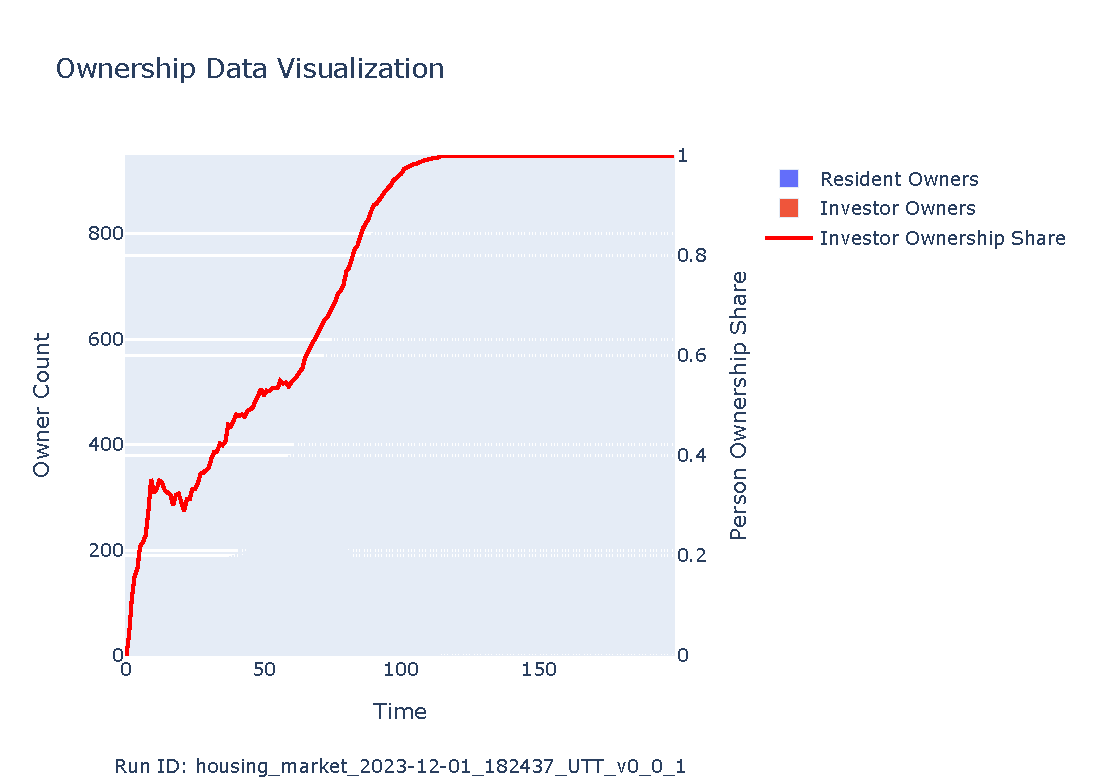
\includegraphics[scale=0.8, trim={0 1cm 0 1.8cm}, clip]{fig/Analysis/Ownership_Data_1.pdf}
    \caption{The transformation from a city of homeowners to a city of tenants in the baseline model}
    \label{fig:Baseline_ownership_trajectory}
\end{figure}

%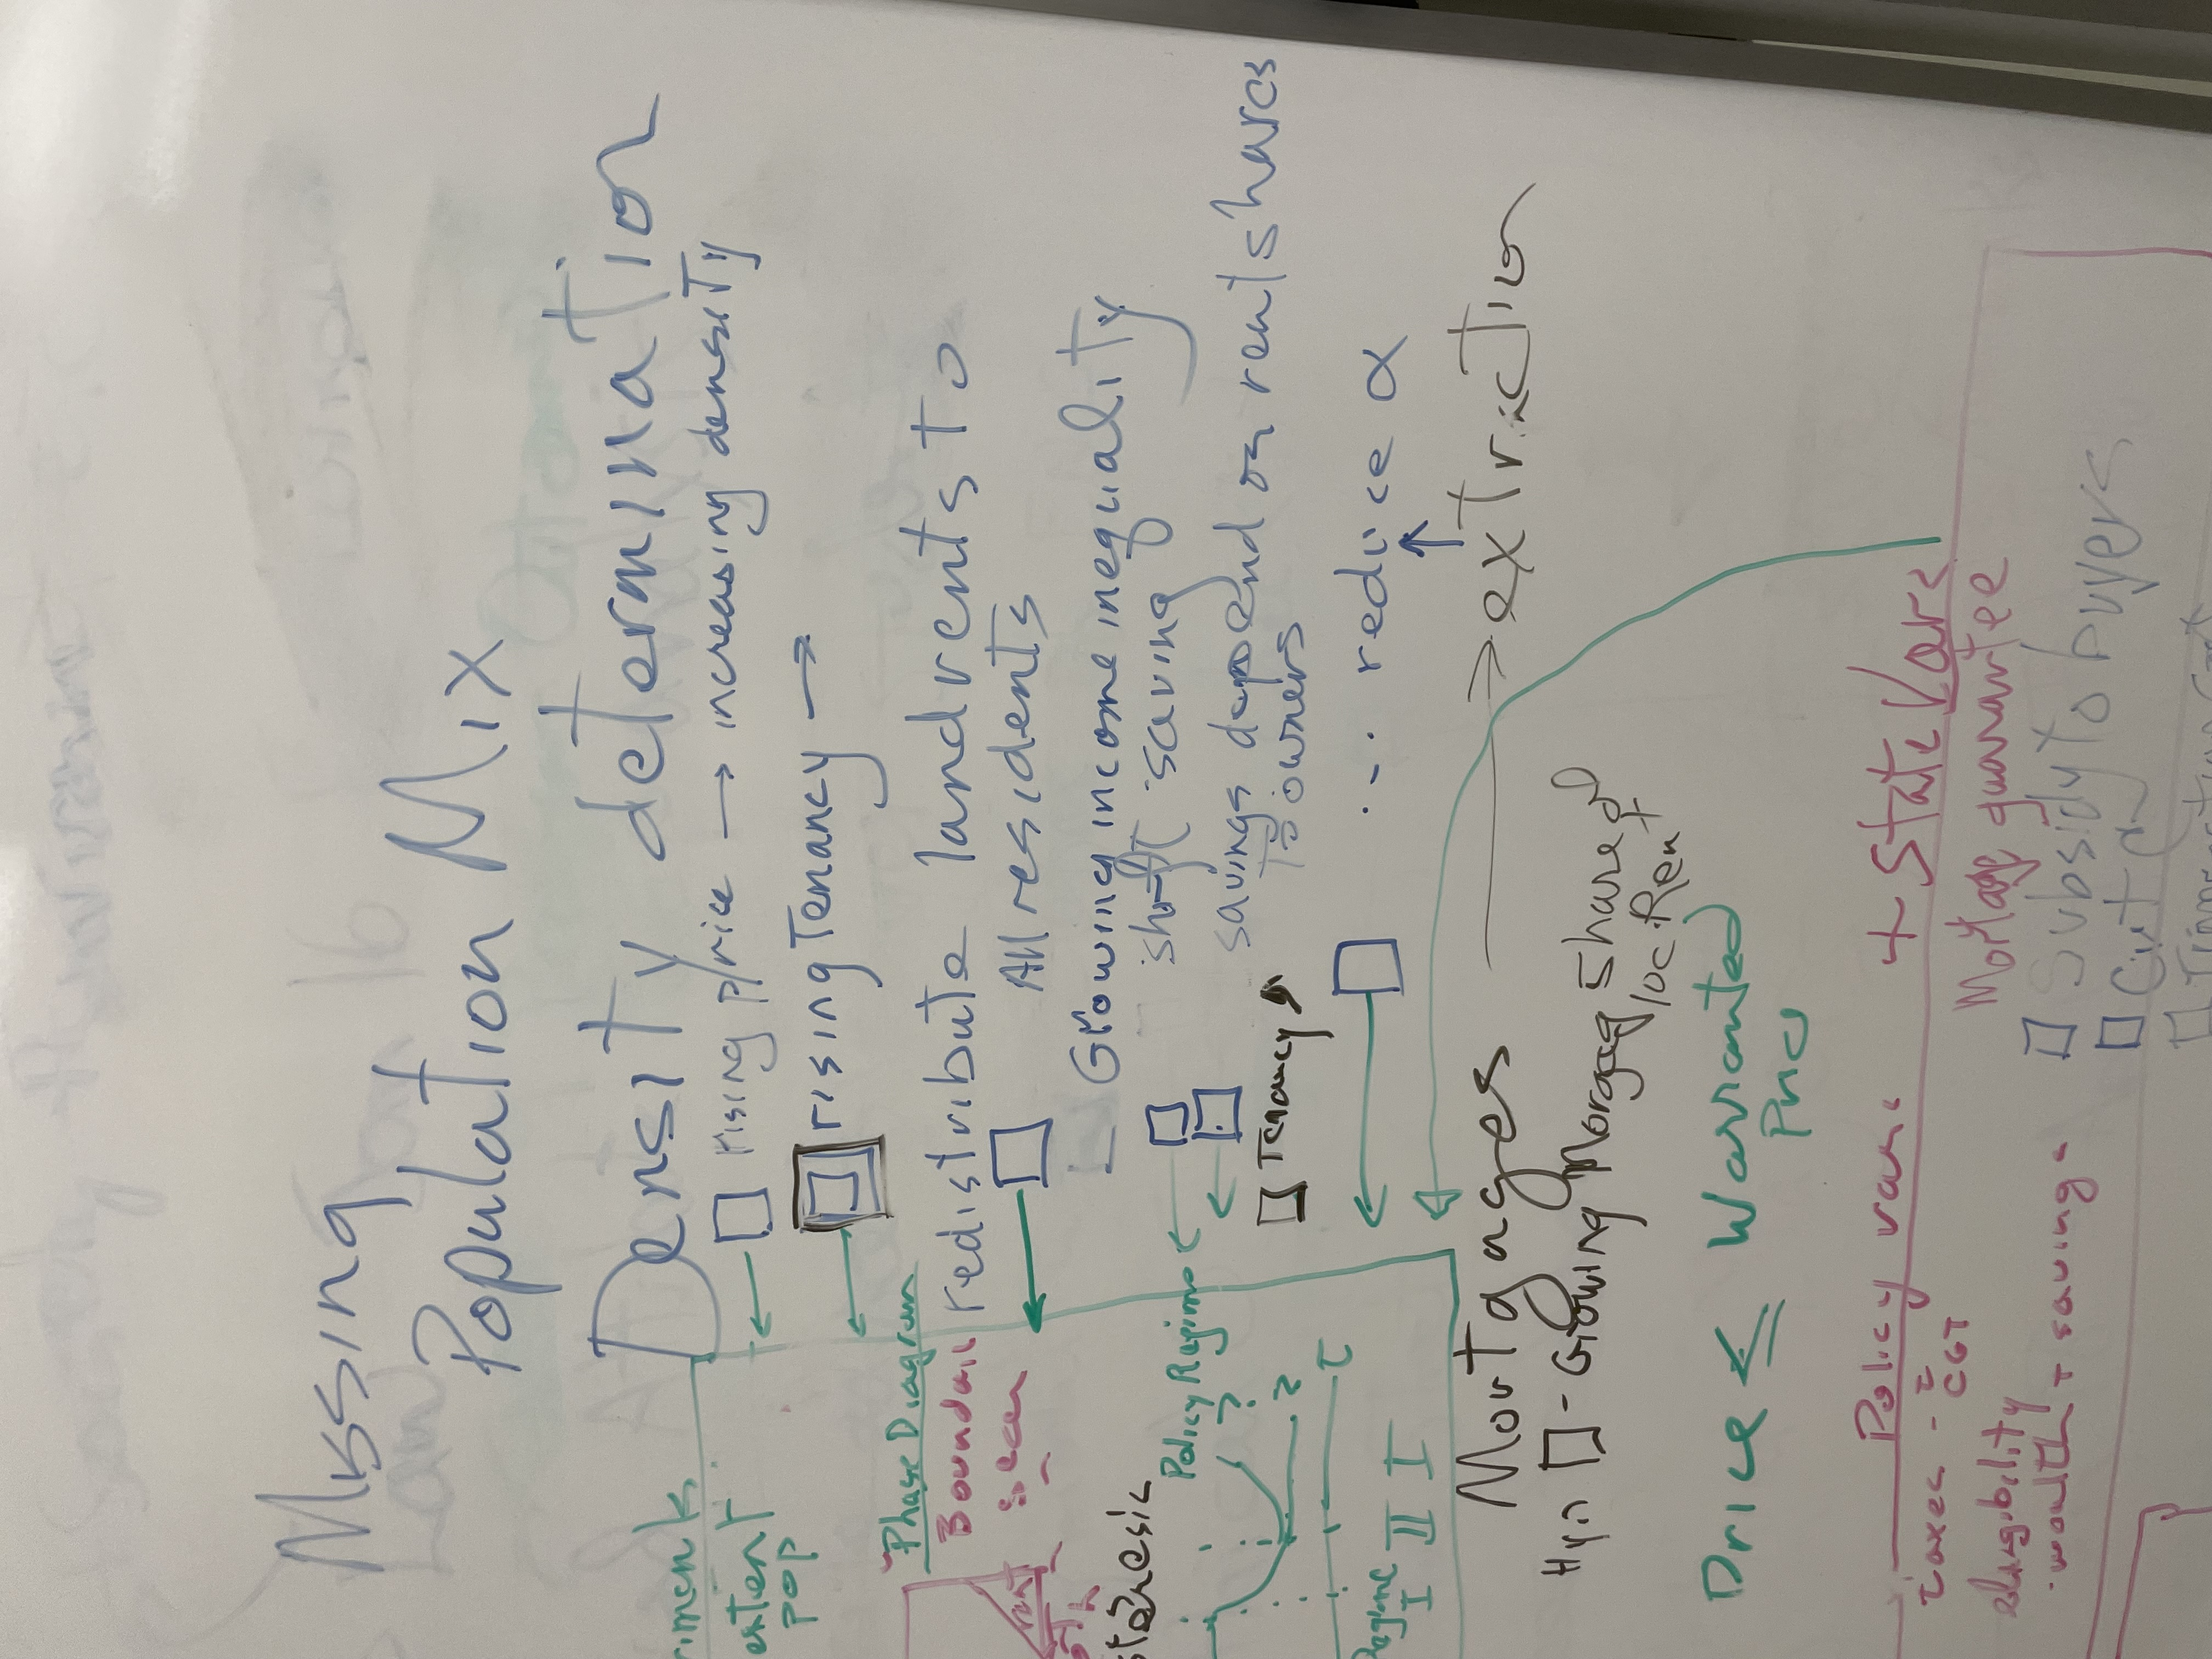
\includegraphics[scale=.5, angle=-90]{fig/IMG_2688.jpg}


%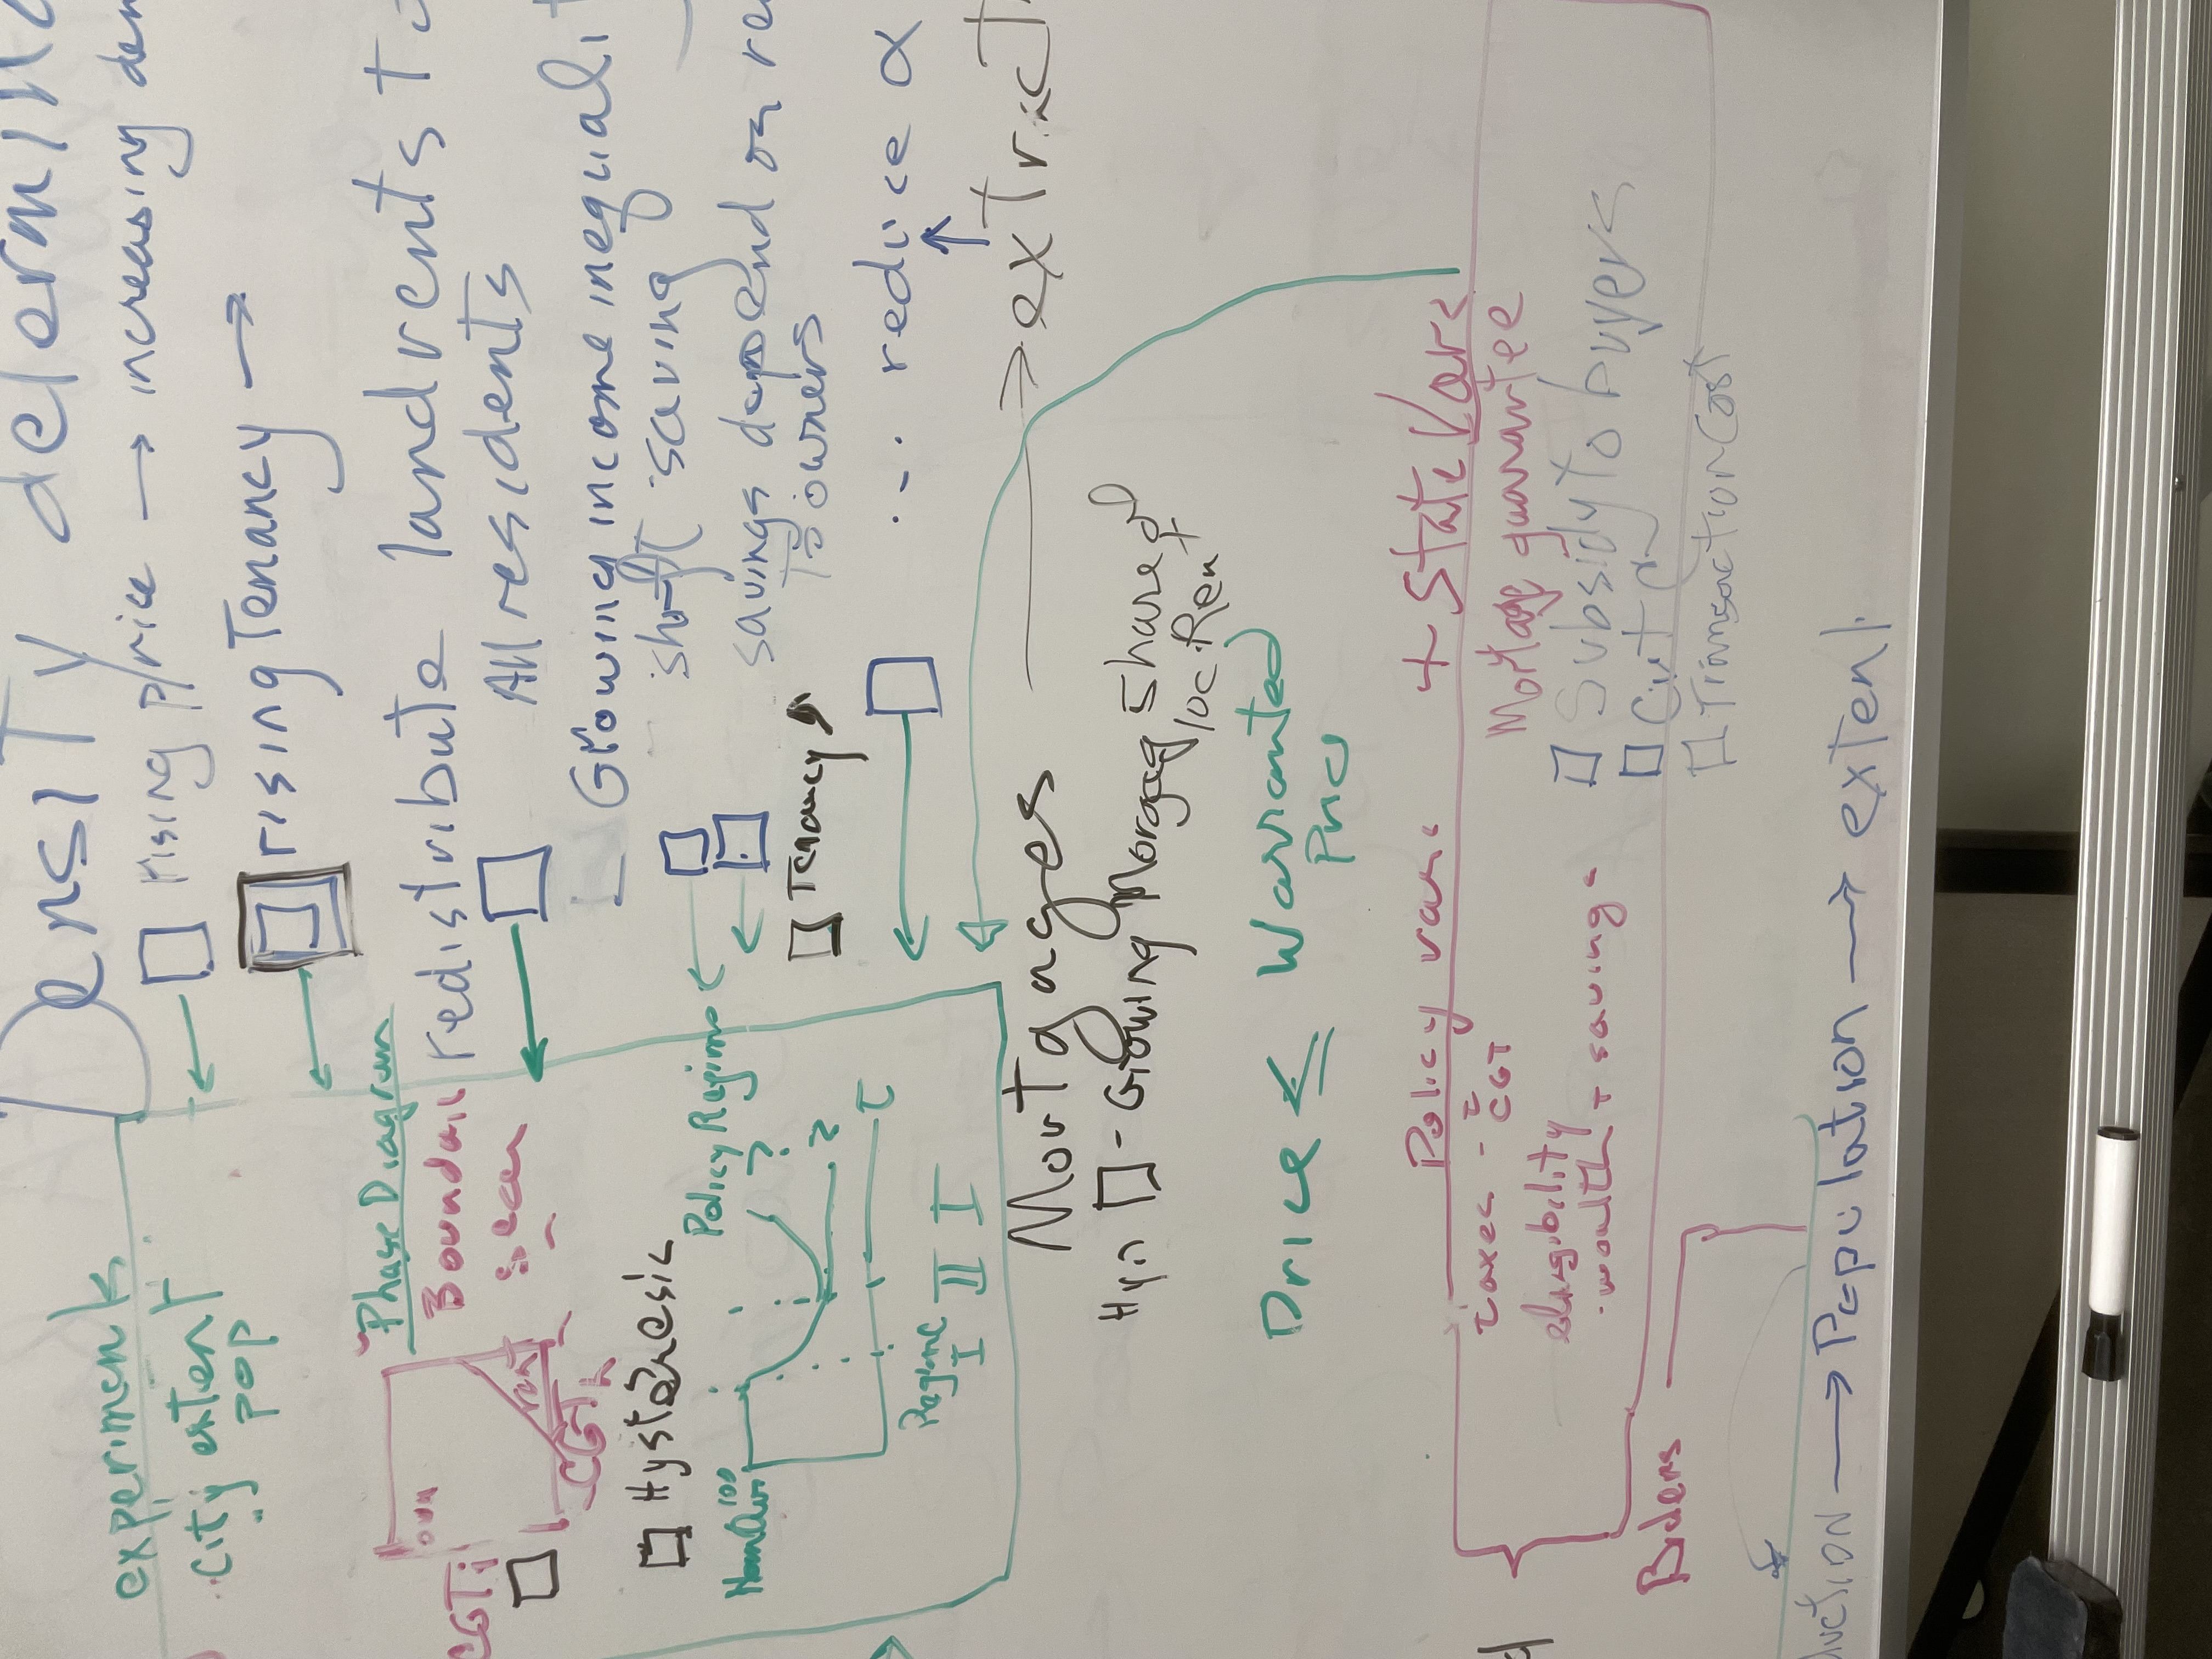
\includegraphics[scale=.5, angle=-90]{fig/IMG_2689.jpg} %Density determination

%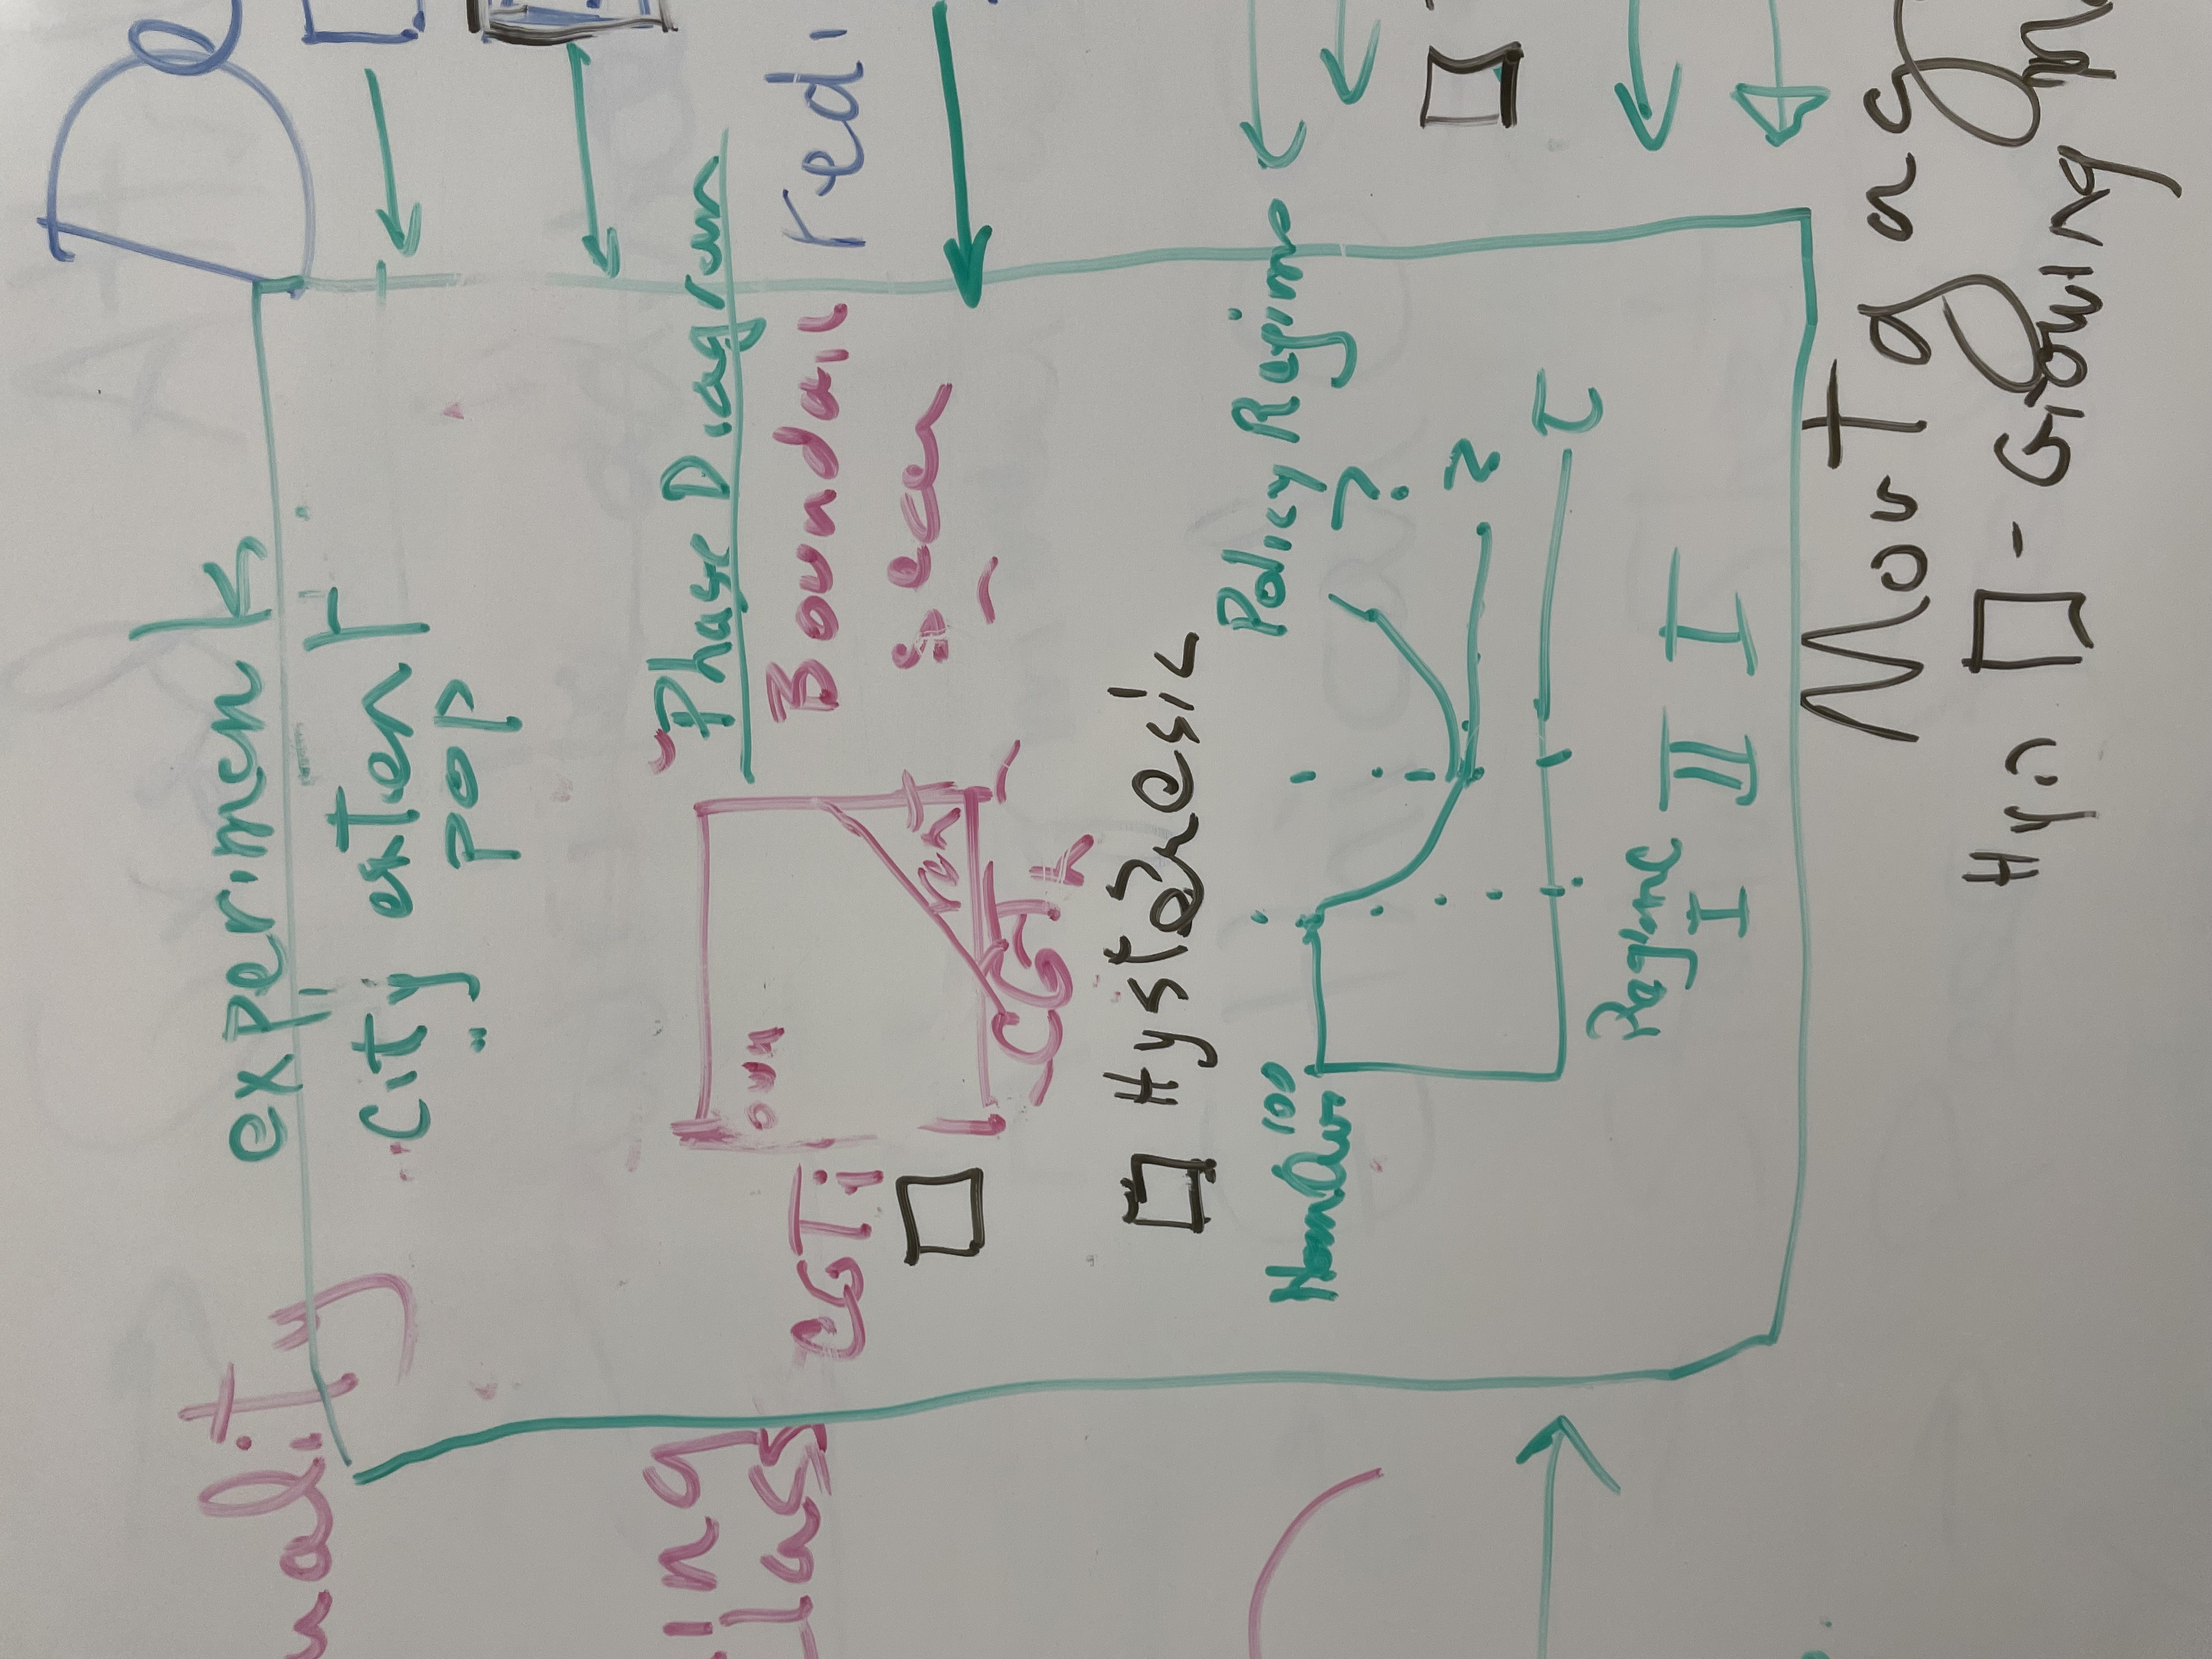
\includegraphics[scale=.5, angle=-90]{fig/IMG_2690.jpg}% 2 FIGURES NEEDED  
%$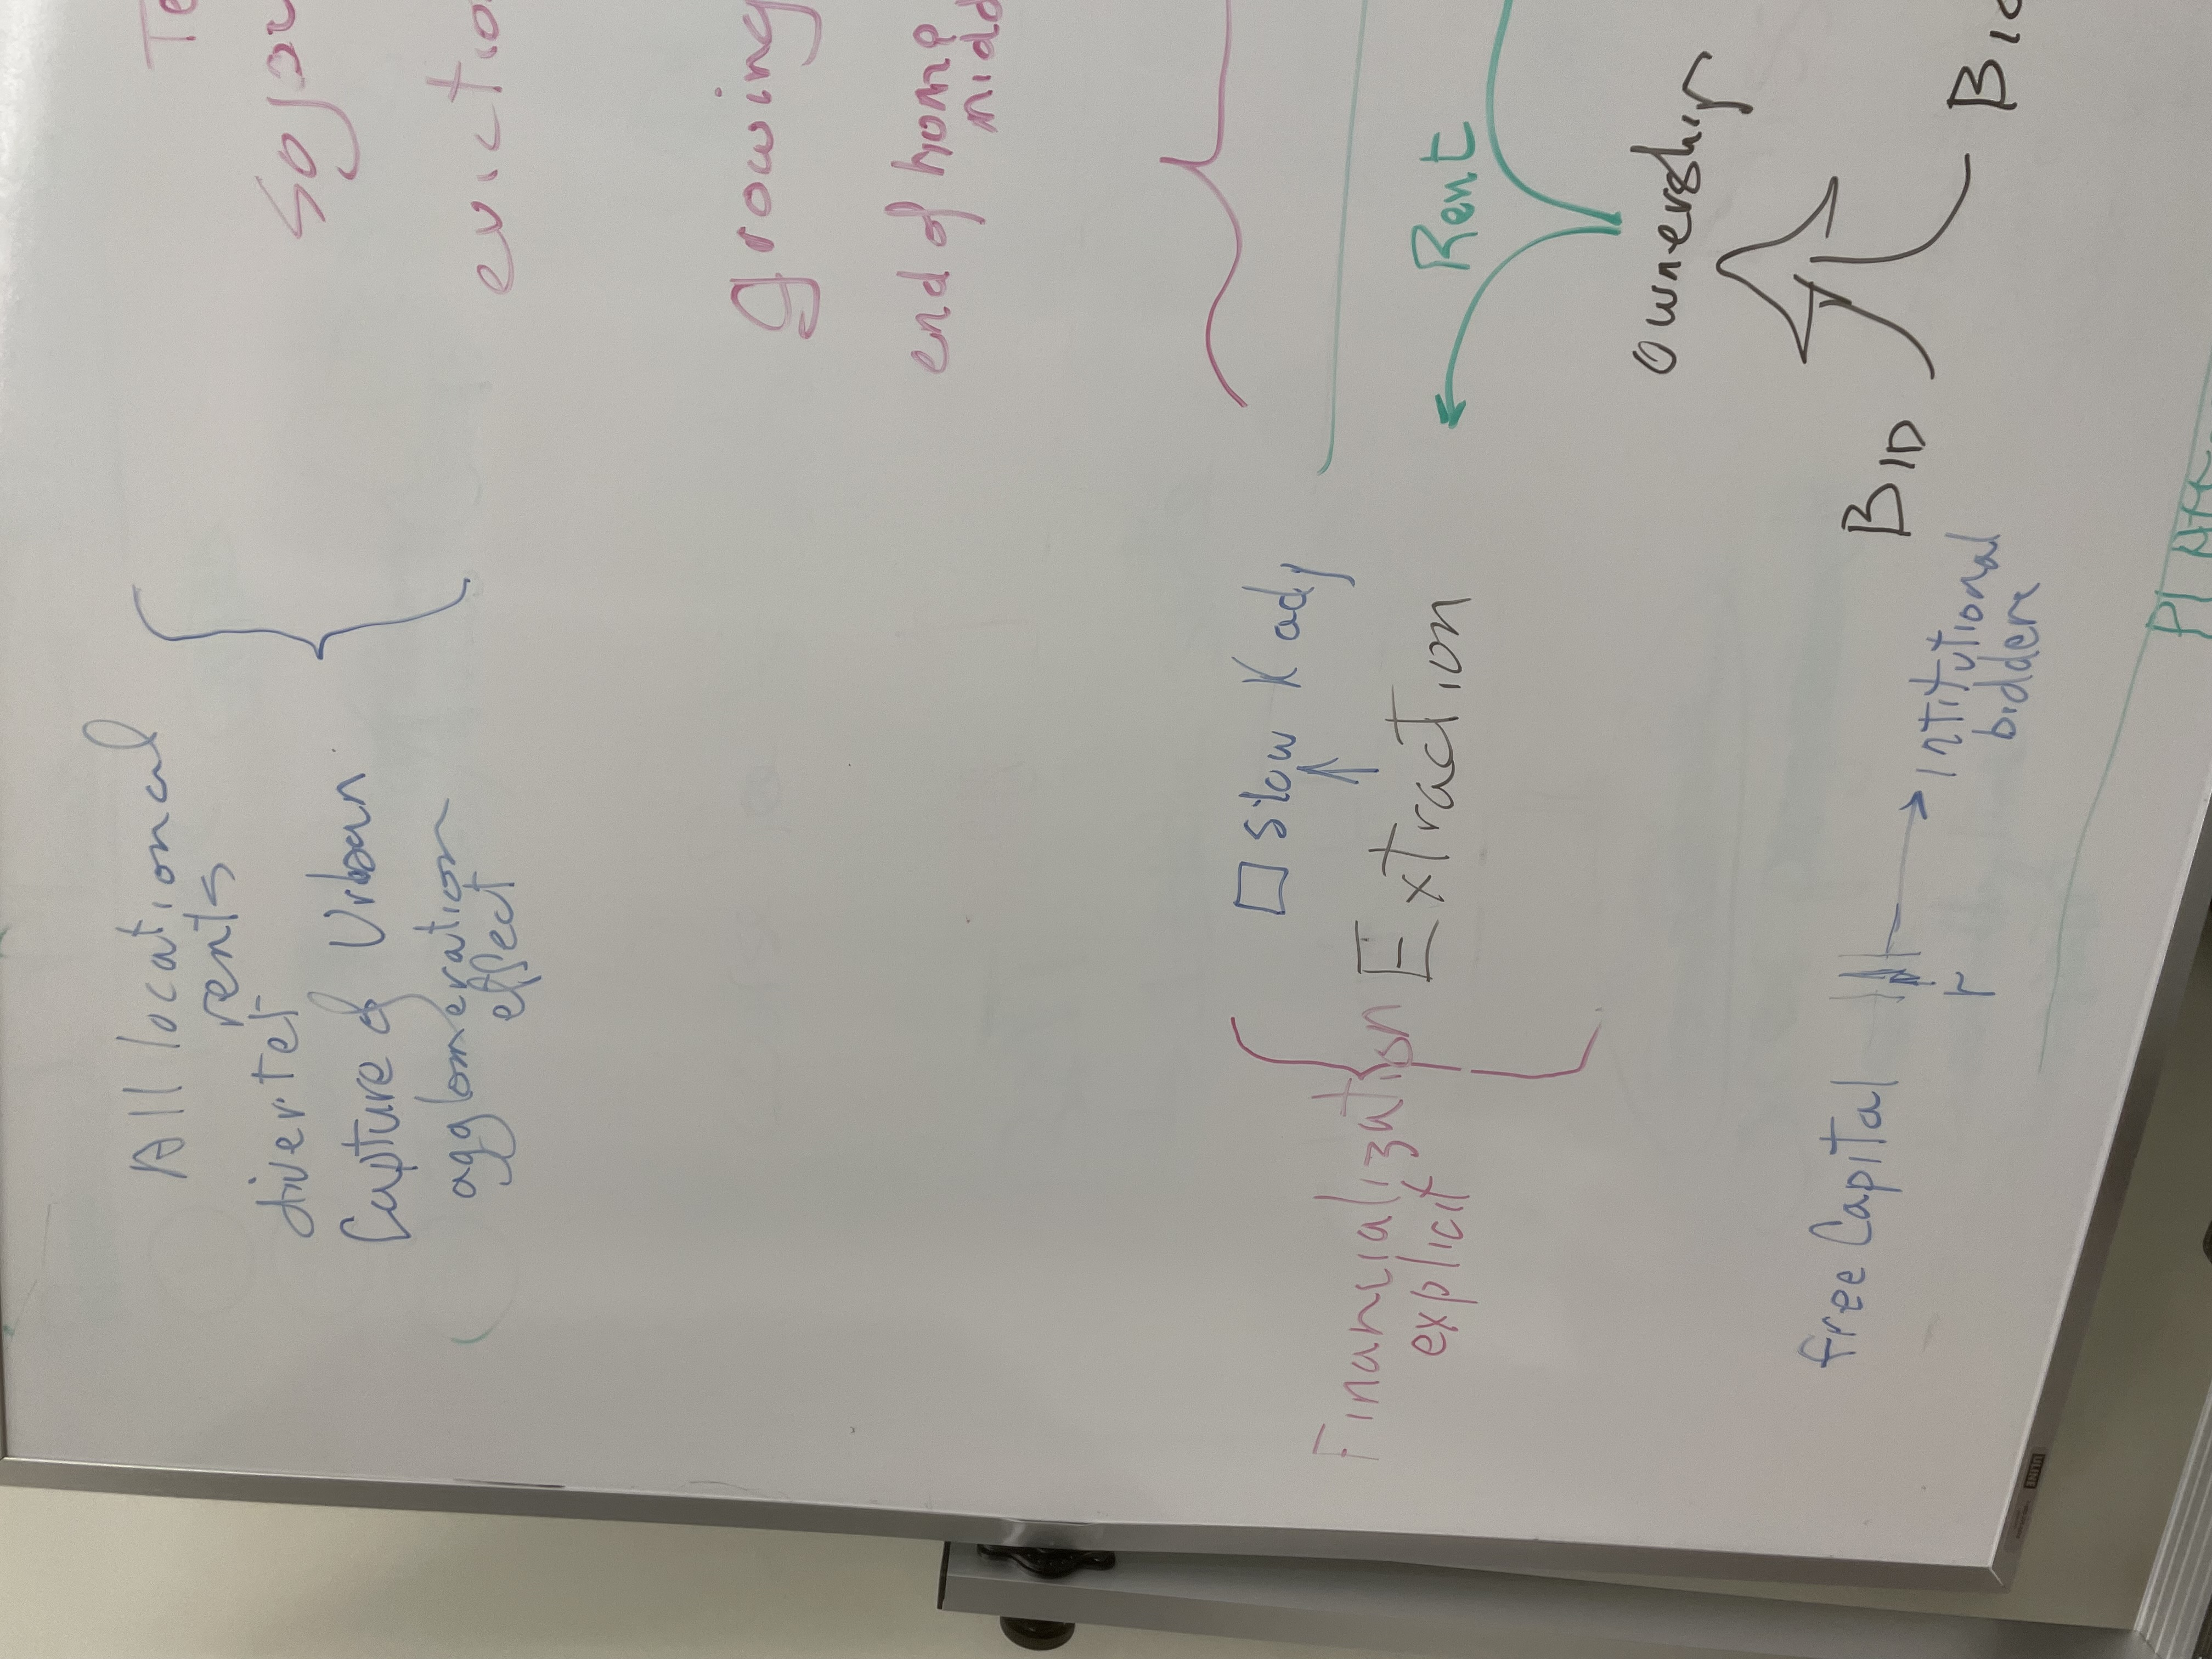
\includegraphics[scale=.5, angle=-90]{fig/IMG_2692.jpg}

%To illustrate a decline in investment we can reduce Kadj.

%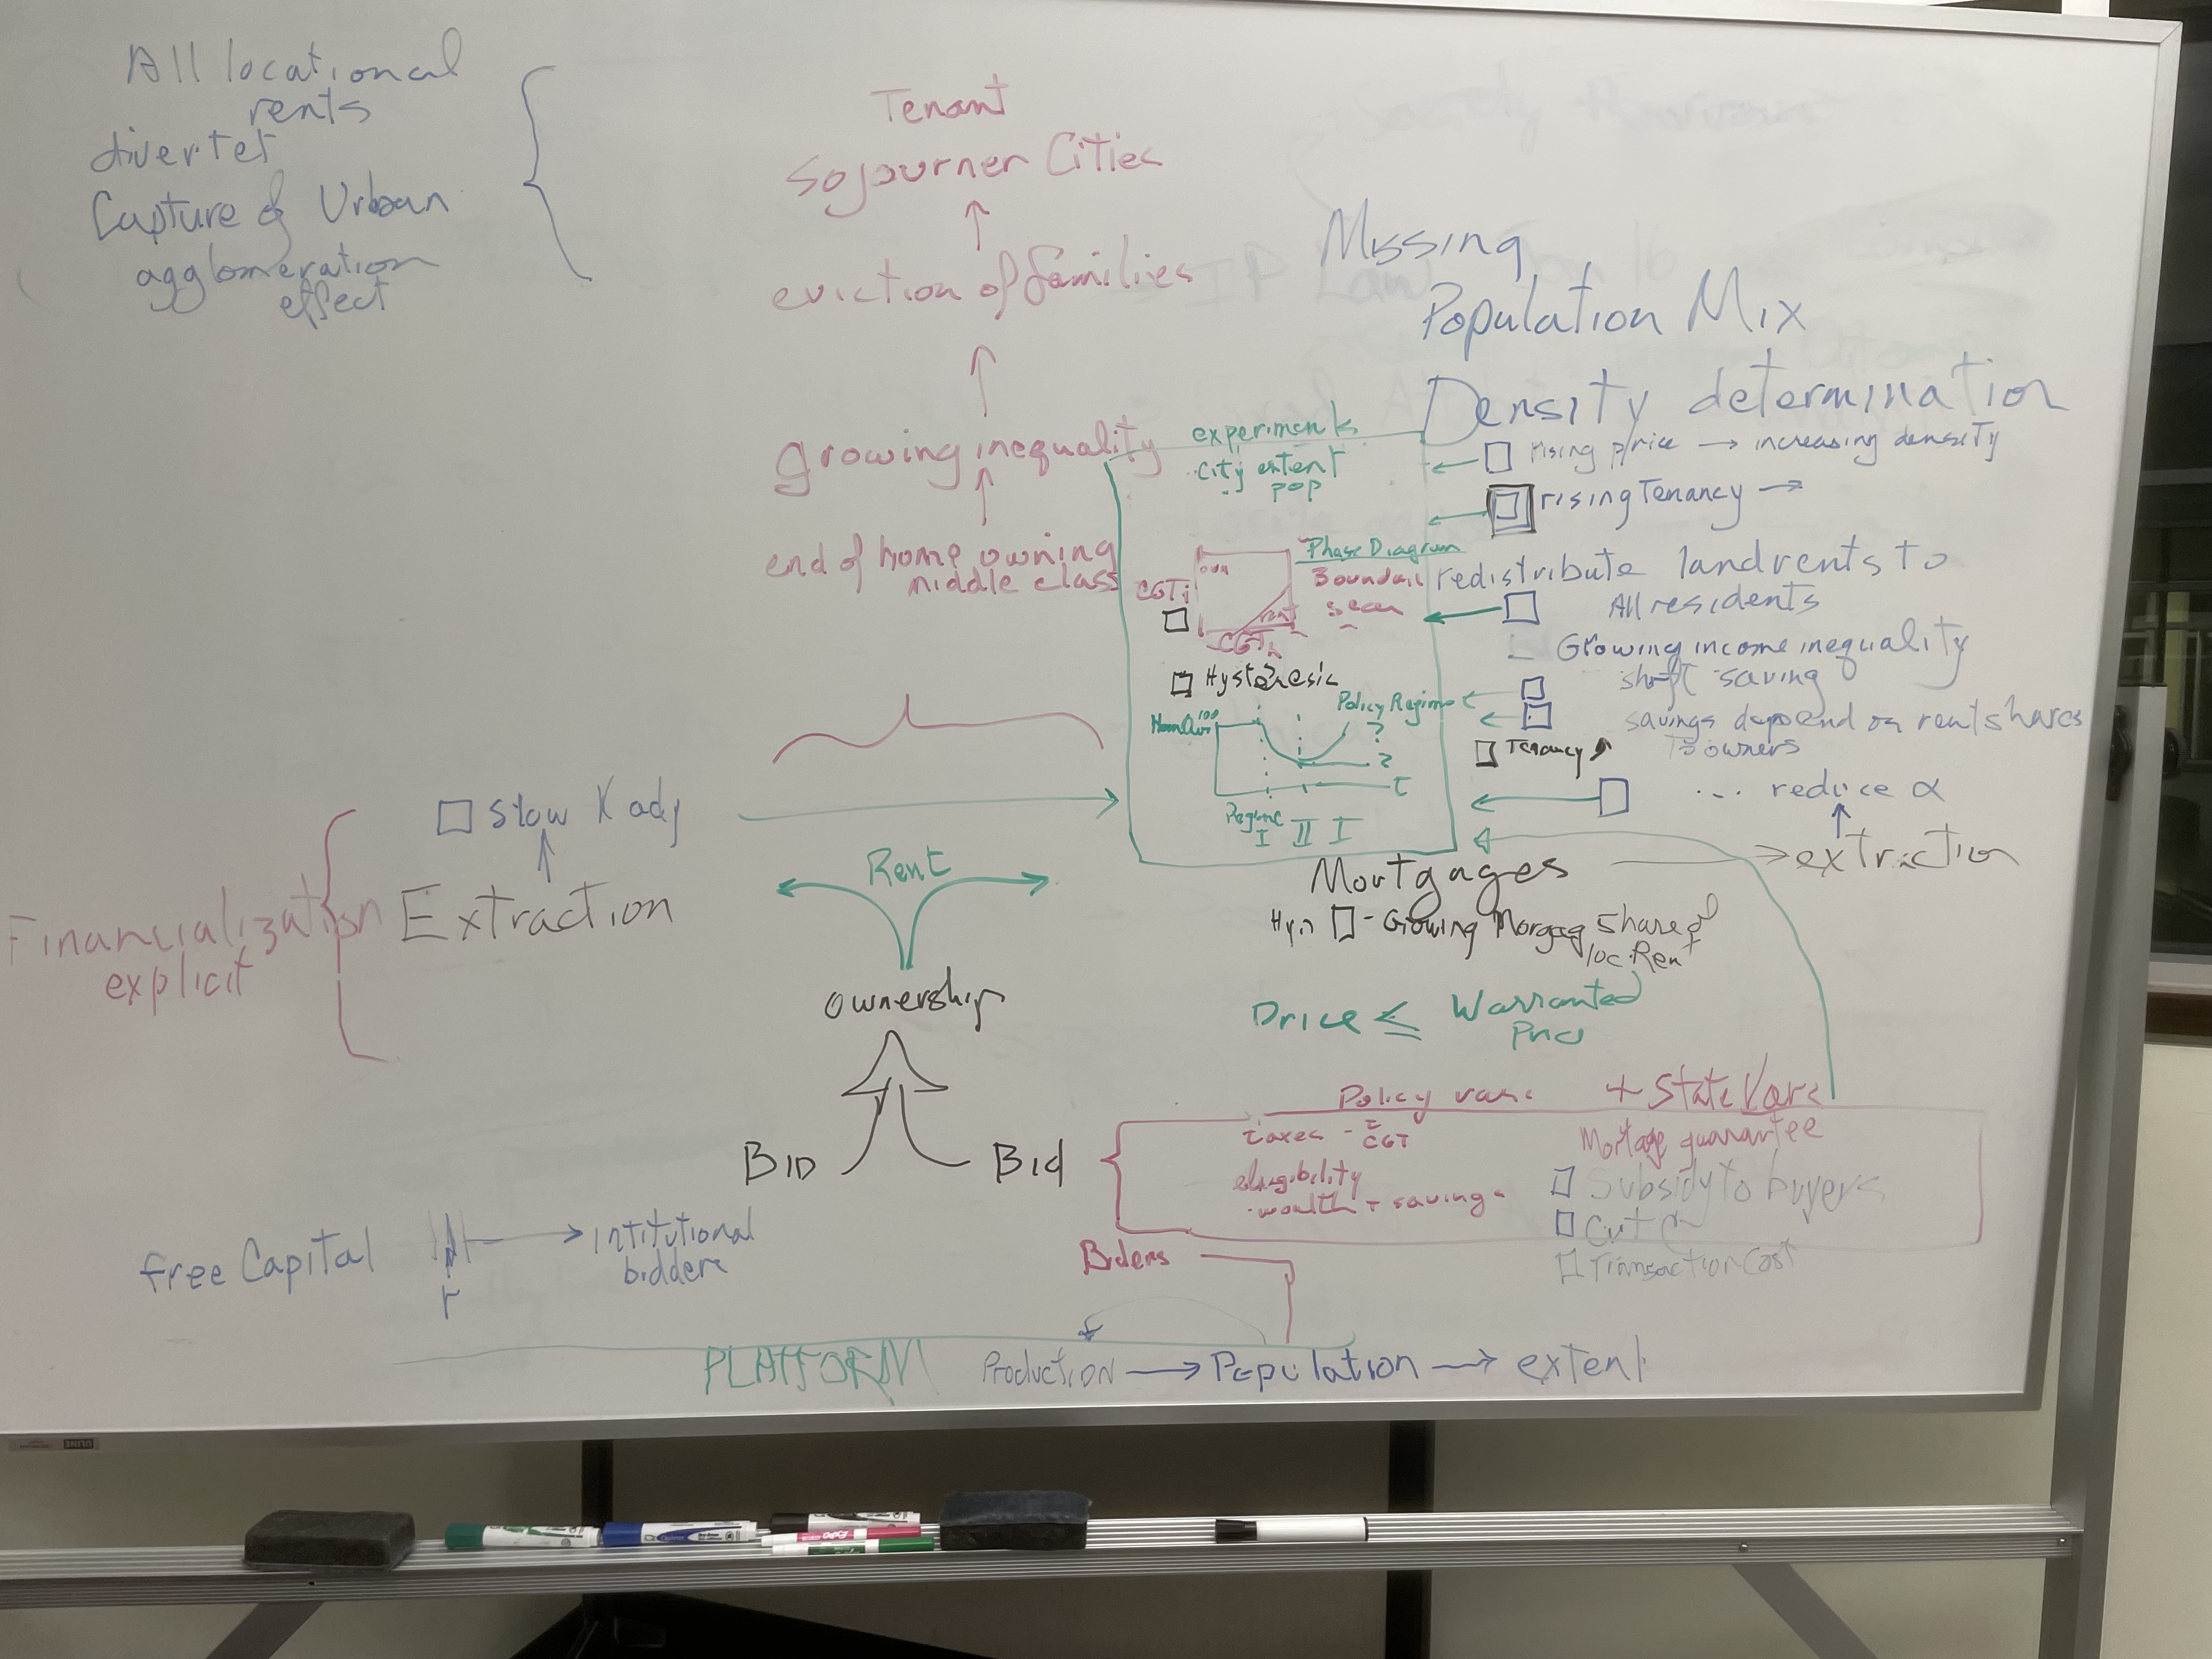
\includegraphics[scale=.5]{fig/IMG_2693.jpg}



The pattern of ownership established as a result plays a crucial role in determining how locational rents within the city are distributed. The consequences of any shift from owner-occupancy to tenancy, shown in red, are dramatic. 
%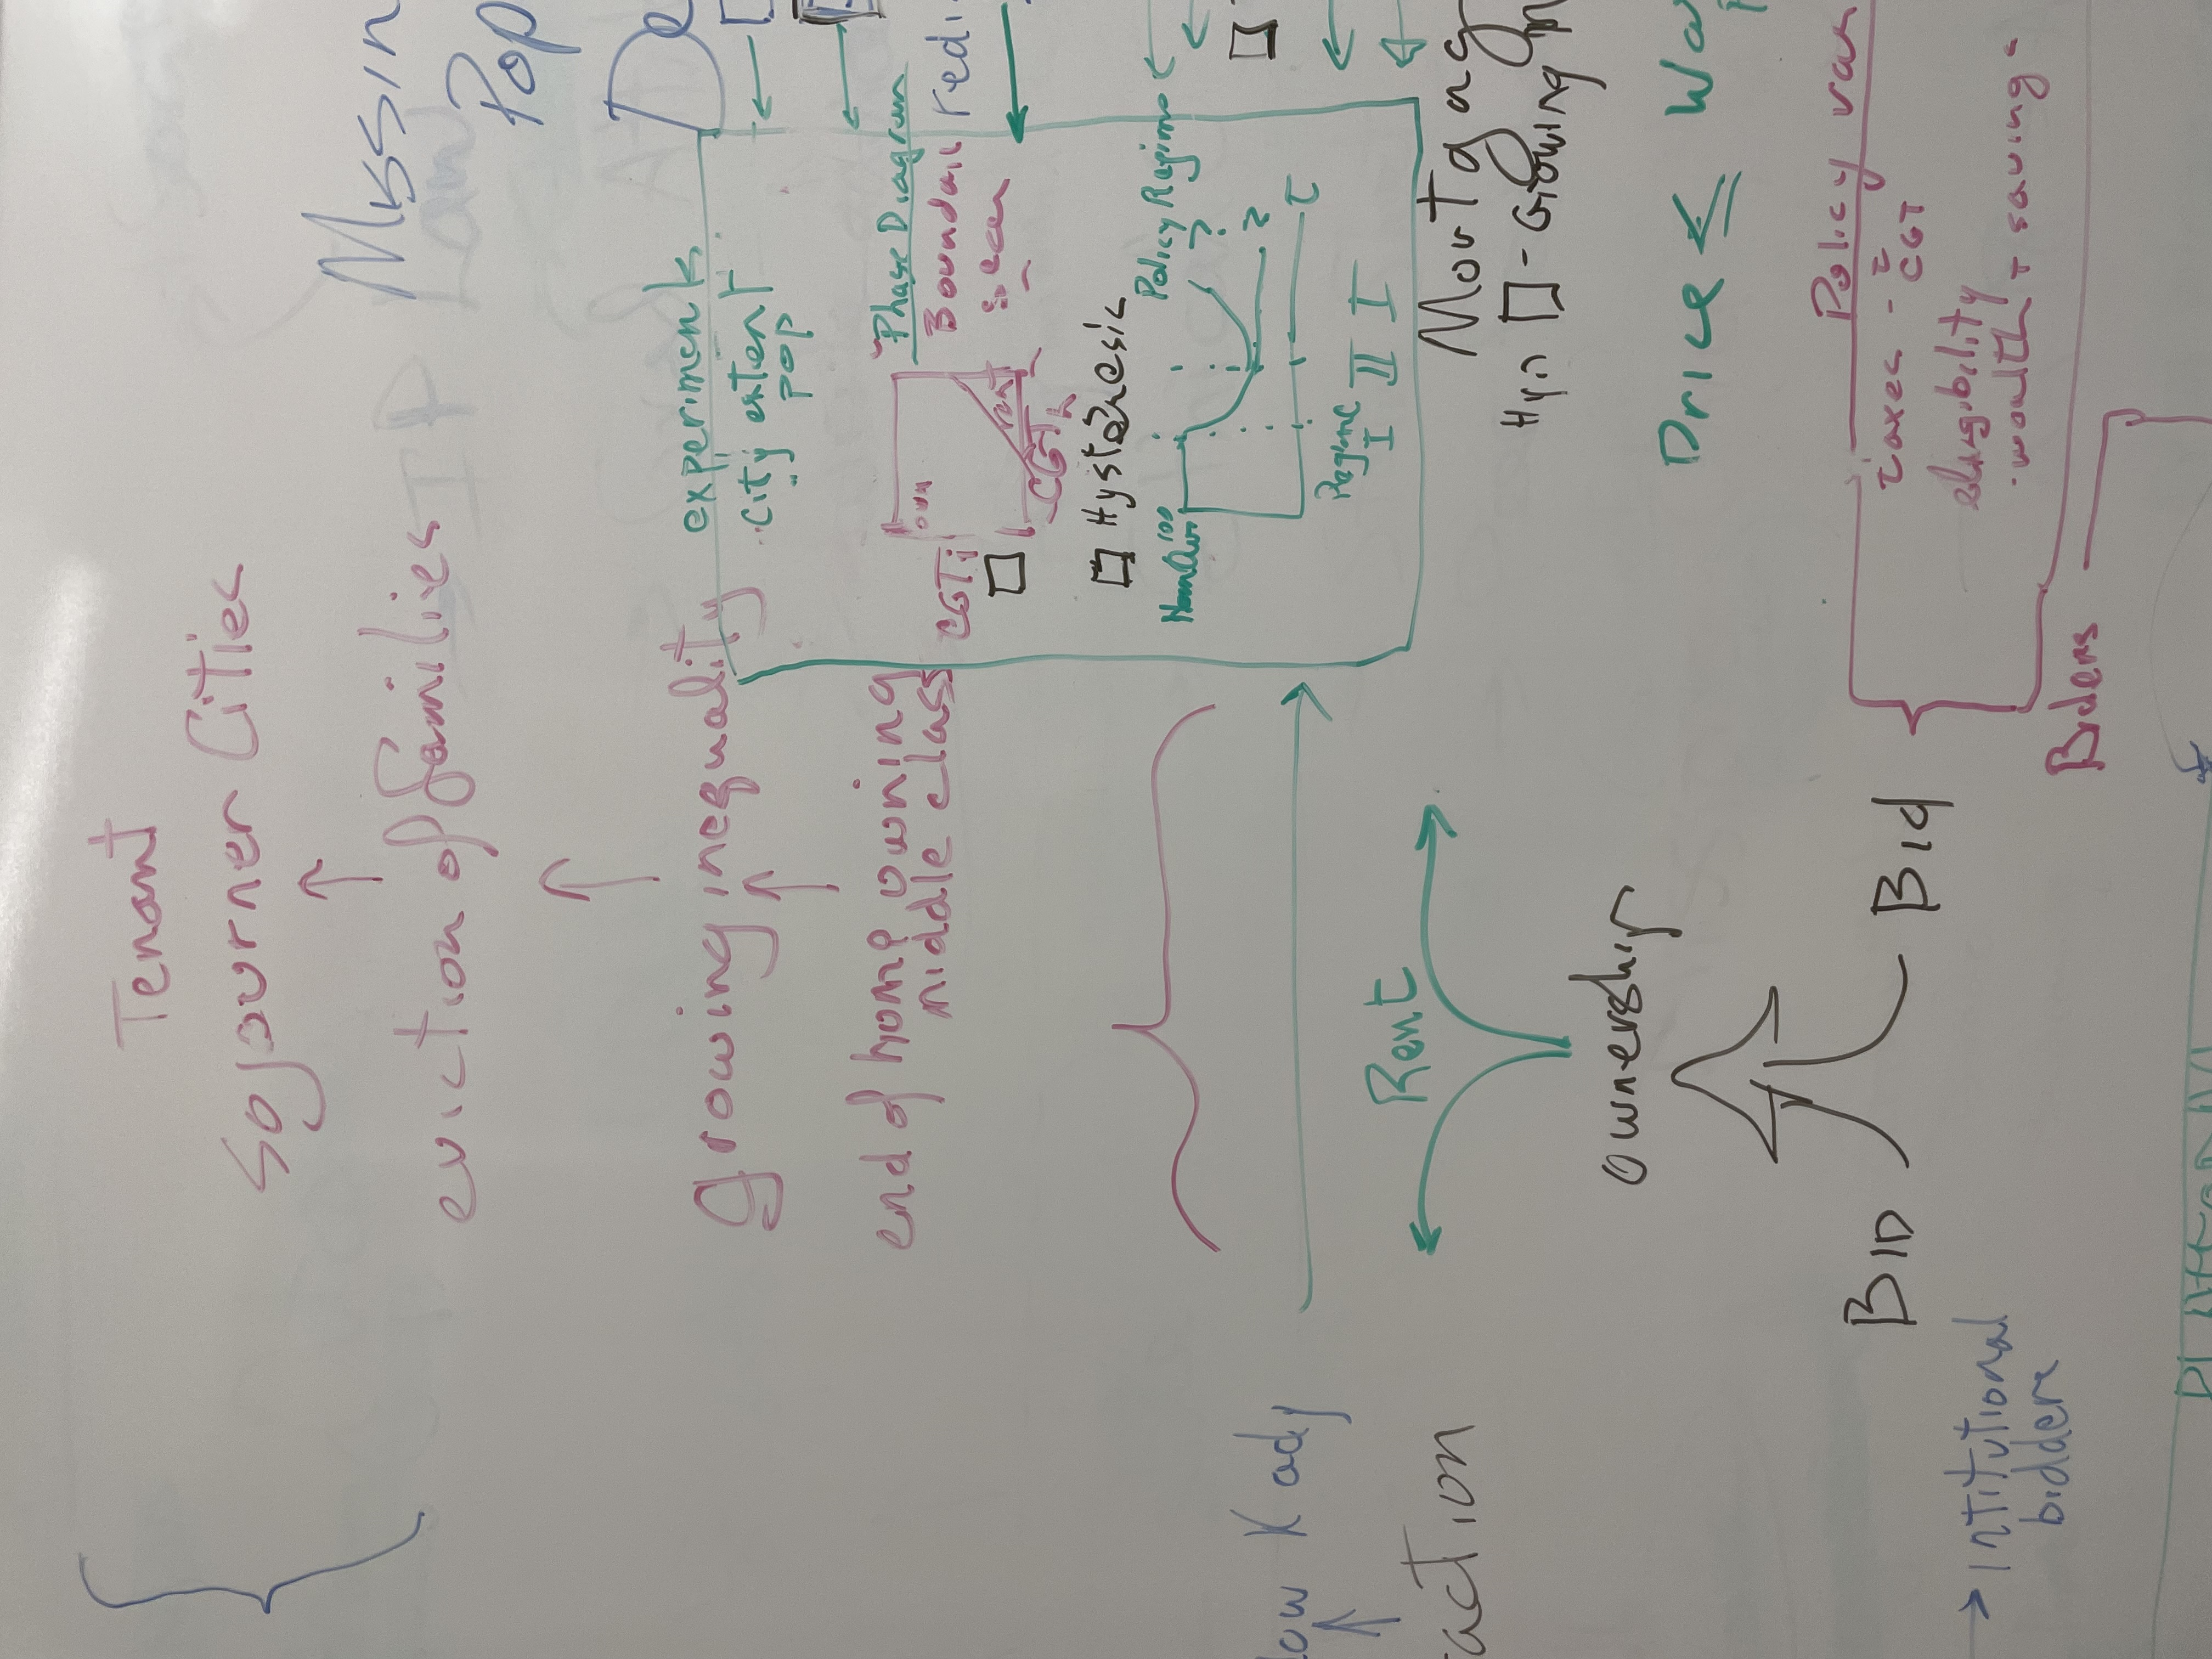
\includegraphics[scale=.5, angle=-90]{fig/IMG_2691.jpg}
The distribution of ownership determines the distribution of the locational land rents, which are the product of agglomeration effects. This general result arises from the specification of the financial sector and the independent behaviour of the agents. It is driven by the operating rules of the financial system. 

Initially, 100\% of locational land rent accrues to residents. In the end, 100\% accrues to the owners of financial capital. Total rents at the end of the period of growth are eight times their initial size.\footnote{Recall that the radius of a circular city is proportional to the wage premium. Rent can be visualized as a cone of volume $\pi r^2 h$ where $h$ is the wage premium. If we double $h$, the volume is increased by a factor of 8.}



\subsection{Policy interventions and ownership}
The tendency for investors to own an increasing share of the housing stock is robust in our model. Can it be affected by public policy? In this section, we look at seven potential policy interventions and their effects on ownership. 

\subsubsection{Capital gains taxation}
Consider a capital gains tax on investors. If capital gains are part of the objective of investors, a capital gains tax will, in theory at least, reduce investor participation. Figure ~\ref{fig:CGinvest_ownership_trajectory} shows this is in fact the case. A capital gains tax on housing investment will have a powerful effect.
\begin{figure}[htb]
    \centering
    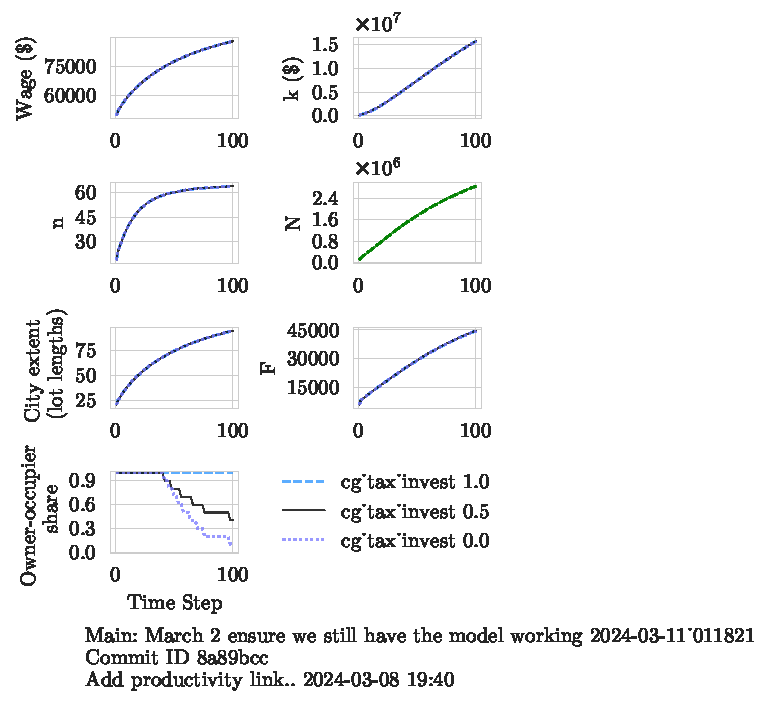
\includegraphics[scale=.8, trim={0 1.4cm 0 0},clip]{fig/cg_tax_invest-Main-_011821.pdf}
    \caption{The effect of a capital gains tax on investors}
    \label{fig:CGinvest_ownership_trajectory}
\end{figure}

The previous result was achieved in a situation where homeowners do not pay a capital gains tax when they sell. This is a policy that has been questioned on ethical grounds because it favours owners over renters.  Figure ~\ref{fig:CGpers_ownership_trajectory} shows that raising the capital gains tax on owner-occupiers will also have a powerful effect. 

\begin{figure}
    \centering
    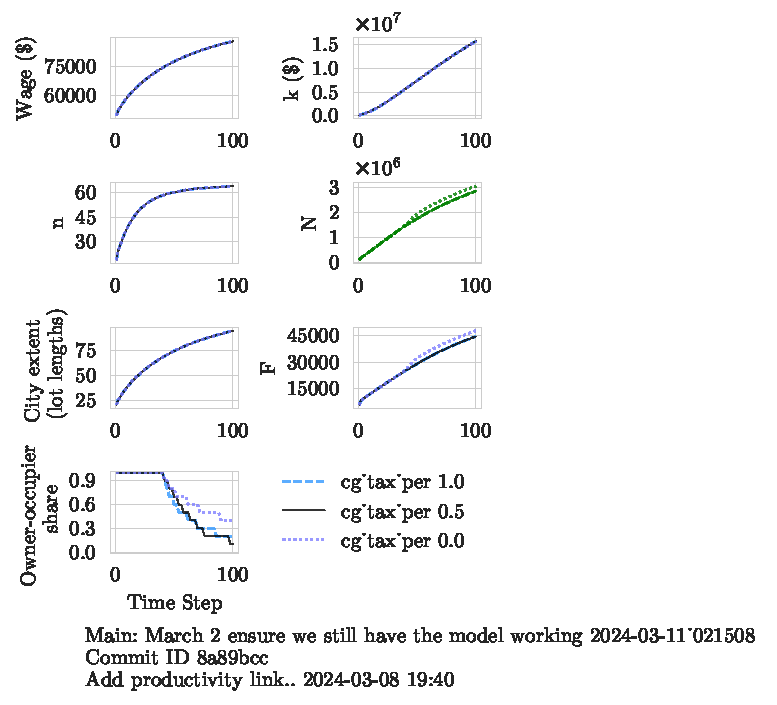
\includegraphics[scale=.8, trim={0 1.4cm 0 0},clip]{fig/cg_tax_per-Main-021508.pdf}
    \caption{The effect of a capital gains tax on homeowners}
    \label{fig:CGpers_ownership_trajectory}
\end{figure}
In this case, the capital gains tax on investors is set at 15\%. The dotted line represents the case with no capital gains tax for homeowners. When the tax is higher than the rate of investors, shown by the solid and the dashed lines,  home ownership falls more than in the base case. In our model, the rents will not fall for tenants, however. Landlords by assumption charge tenants the full locational value, and that does not depend on whether there are capital gains for property owners.

%%%%%%%%%%%%%
\newpage

\subsubsection{The cost of capital for investors}
% 'r_investor': [0.2, 0.1, .05] has set up for morning
Figure ~\ref{fig:capital_ownership_trajectory} shows the effect of increasing capital costs for investors. Higher capital cost might be expected to slow the rate of housing acquisition. Surprisingly, it appears to increase the speed at which investors purchase but it does not affect not the final level of investor ownership.  In addition, it appears to decrease population, suggesting that the cost of acquiring housing rises. The cost of capital for investors is not an obvious policy tool, so we don't think this result is of great interest politically, but it warrants further study.
\begin{figure}[h!t]
    \centering
    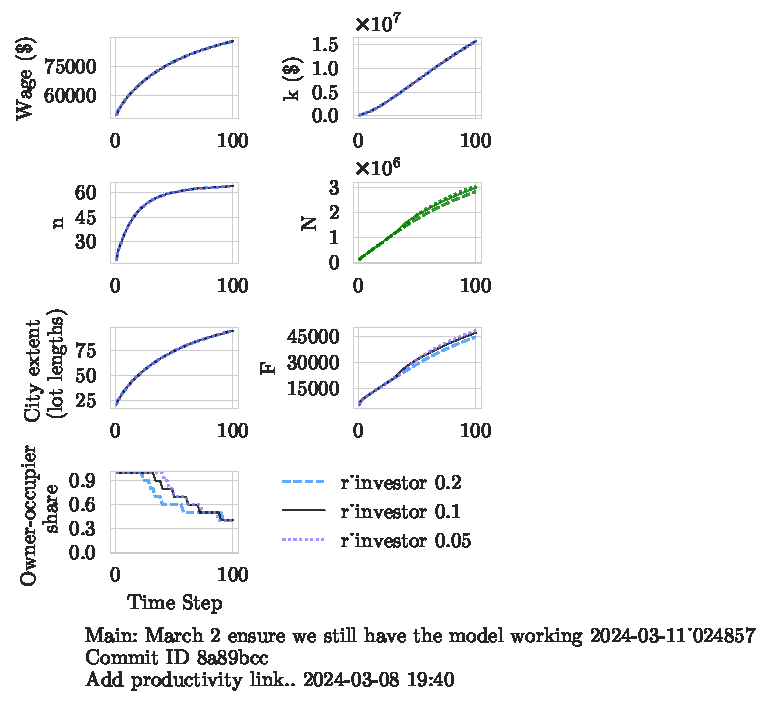
\includegraphics[scale=.8, trim={0 1.4cm 0 0},clip]{fig/r_investor-Main-024857.pdf}
    \caption{The effect of raising capital costs}
    \label{fig:capital_ownership_trajectory}
\end{figure}

\newpage
\subsubsection{Transportation costs}
Roads and road congestion as well as the transit system are public responsibilities. They affect the cost of transportation. Can reducing the cost of transportation affect the ownership ratio. In Figure~\ref{fig:c_ownership_trajectory}, we reduce transportation costs for everyone by 40\%. 

%This is what we expect in the Alonzo model within this model.
We expected the city would grow faster and get larger with lower transportation costs. This effect was indeed observed. 
% 'c': [500, 300],

Less obviously, lower transportation costs also served to  to decrease the home-ownership ratio. The reduction in transportation costs leads to an increase in land rents, and the increase in land rents increases the rate of increase of property prices, leading to higher expected capital gains and ultimately less private ownership. 




\begin{figure}[h!t]
    \centering
    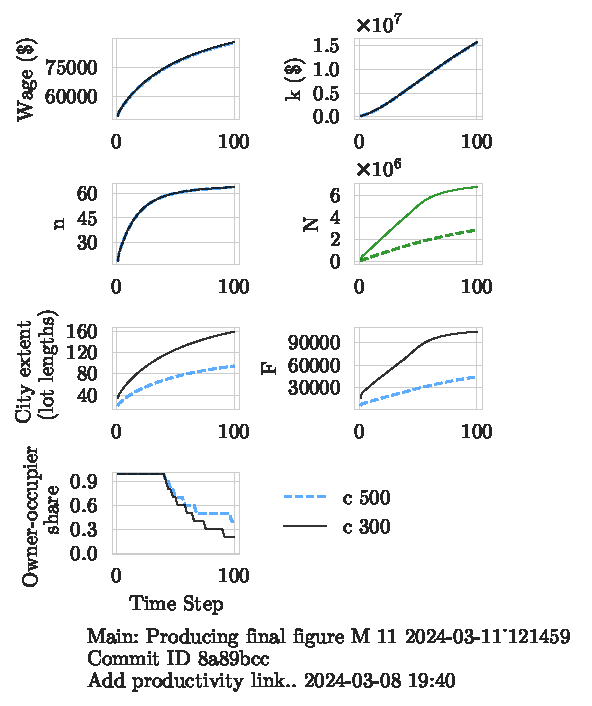
\includegraphics[scale=.8, trim={0 1.4cm 0 0},clip]{fig/c-Main-121459.pdf}
    \caption{The effect of decreasing transportation costs}
    \label{fig:c_ownership_trajectory}
\end{figure}


\newpage
\subsubsection{Density}
% 'density': [100, 150]
Density is a policy variable that is much discussed. Increasing density is proposed as a way to increase housing availability and the ability of people to buy homes. Our results indicate that the effect of density on city population is significant but it has no effect on city extent and no effect on the ownership ratio. The first two results are expected, the third less so but easily explained. 

Essentially the share of homeowners is not affected, only the number of homes is. Since rent per unit is unchanged, density alone does not affect the relative advantage of new home buyers and investors, leaving the ratio constant. There are more homes, however, and, since the ratios are consistent, more home-owners. 

\begin{figure}[h!bt]
    \centering
    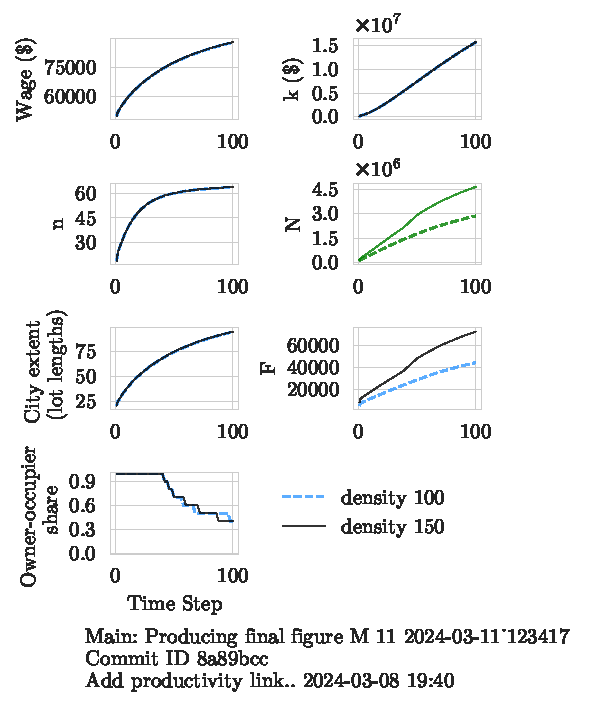
\includegraphics[scale=.8, trim={0 1.4cm 0 0},clip]{fig/density-Main-123417.pdf}
    \caption{The effect of increasing density}
    \label{fig:density_ownership_trajectory}
\end{figure}


\newpage

\subsubsection{Cost of financing's dependence on borrower's wealth}
Wealth sensitivity in our model is a parameter of the banking system. It determines how easy it is for people with limited assets or income to get a mortgage. A higher value is more restrictive:  makes it harder for an asset-poor person to get a mortgage.

A restrictive mortgage regime slightly reduces labour supply and city population. It has no noticeable effect on the ownership ratio. Since the purpose of a restrictive policy is to reduce defaults and bankruptcies, the small impact on other variables suggests that as a policy it can be adopted without needing to consider the economic impacts on the city. 
% 'wealth_sensitivity': [0.15, 0.1, 0.5]

\begin{figure}[h!bt]
    \centering
    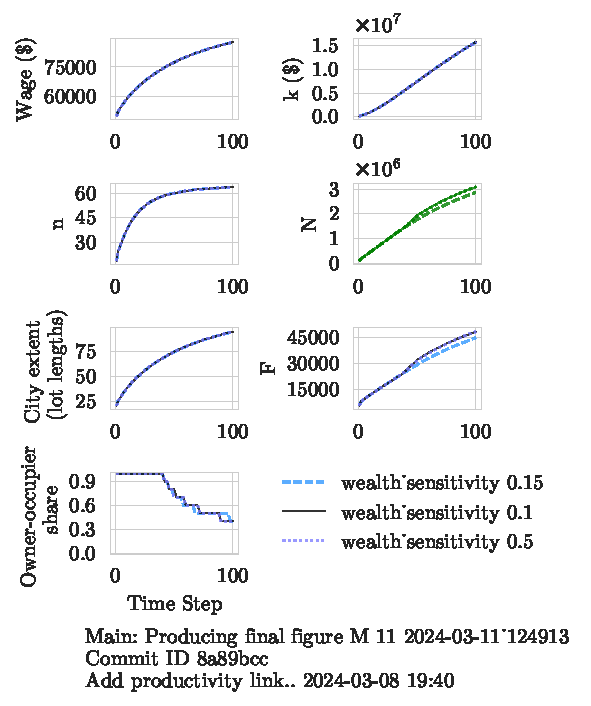
\includegraphics[scale=.8, trim={0 1.4cm 0 0},clip]{fig/wealth_sensitivity-124913.pdf}
    \caption{The effect of wealth sensitivity of mortgage access}
    \label{fig:wealth_sensitivity_ownership_trajectory}
\end{figure}

\newpage

\subsubsection{The property tax rate}

The property tax rate variable is a matter for policy debate because there are good reasons to think, first, that property taxes are a barrier to ownership, and second, that the property taxes are not paying all the costs of public infrastructure and services to homeowners, leading to significant inequities.

% 'property_tax_rate': [0.1, 0.05, .01] k doing}
\begin{figure}[h!tb]
    \centering
    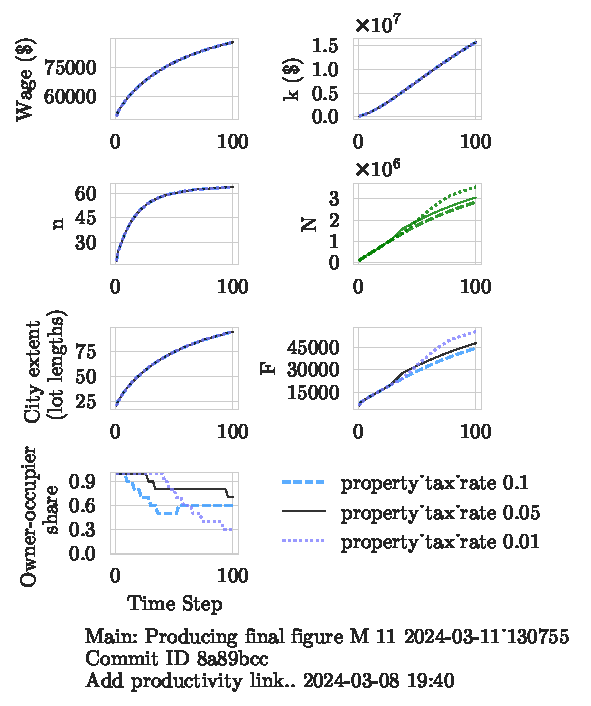
\includegraphics[scale=.8, trim={0 1.4cm 0 0},clip]{fig/property_tax_rate-Main-130755.pdf}
    \caption{The effect of property tax rates}
    \label{fig:property_tax_ownership_trajectory}
\end{figure}

\section{Results including a linkage tying financialization back to productivity}

In this section, we use our model to explore some implications of a hypothetical link between financialization of an urban housing market and the urban production economy. We are not trying to demonstrate that there is a link whereby financialization affects urban productivity. The literature make a strong case that there is a linkage and provides a transmission theory through several mechanisms so we have built the link in to see the implications and look at what is likely to matter as a result of the transition in ownership pattern.

A simulation of this linkage is illustrated in Figure~\ref{fig-impact-channel-example}. The finance-driven change in ownership share shown in the lower panel transforms a city of homeowners into a city of renters over the course of a lifetime. It also has, as we hypothesized, substantial economic implications. The change in the the class structure of the city induces a decline in worker productivity and capital investment, resulting in reduced firm size and a reduction in the number of firms, as well as an overall reduction in population. 

Declining productivity is the primary channel for this change, which pulls down the wage and the other population variables. The change is amplified by the resulting reduction in aggregation effects.  If the linkages we have hypothesized exist, the result of financialization would be a poorer society. 

\begin{figure}[h!tb]\label{fig-impact-channel-example}
    \centering
    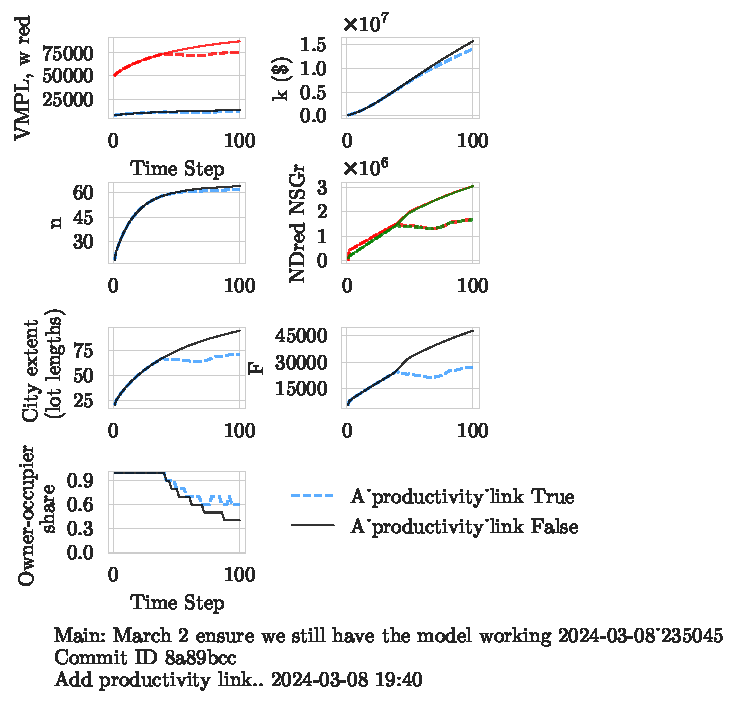
\includegraphics[scale=1, trim=.25cm 2cm .25cm .25cm, clip]{fig/productivity_link.pdf}
    \caption{Illustrating the impact of financialization on an urban economy}
\end{figure}
This is, to our knowledge, a new result, although it is consistent with fundamental urban theory and with the trends we see today in the urban system. The new component in our result is the formal linkage of the financialized housing market to urban productivity.

We do not have empirical estimates about the strengths of the channels through which the productivity effect would work, however, so only the direction of the impacts illustrated should be taken seriously without further empirical work.  


Assuming there are linkages connecting financialization to productivity, it is important to ask if there are policy implications. Figure~\ref{Productivity_link_and_CG} indicates the effect of a 100\% capital gains tax on land speculation. 

\begin{figure}[h!tb]\label{fig-Productivity_link_and_CG}
    \centering
    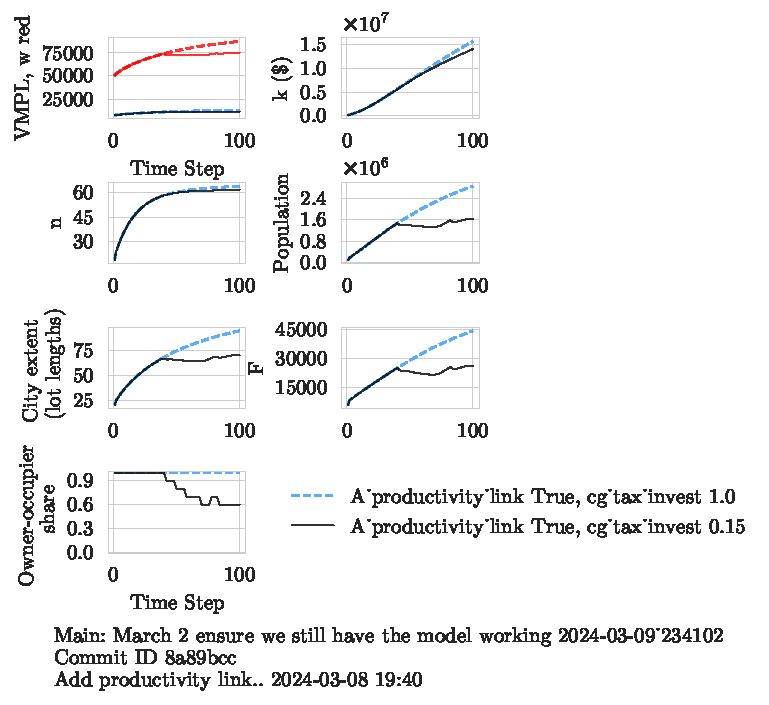
\includegraphics[scale=1, trim=.25cm 2cm .25cm .25cm, clip]{fig/Productivity_link_and_CG.pdf}
    \caption{The corrective effect of a capital gains tax}
    \label{fig:Productivity_link_and_CG}
\end{figure}

The figure shows that a 100\% capital gains tax on land speculation returns the city to its pre-financialization path, indicated by the solid line. In the housing market it has an `excess' effect, eliminating investor participation in the market, shown by the dashed line, and leading to higher rates of home ownership. 

% {\newpage\thispagestyle{empty}
% \vspace{-1.5cm}
\begin{figure}[h!tb]\label{fig-impact-channels}
%\vspace{-1cm}
\begin{adjustwidth}{-0.24\textwidth}{-0.24\textwidth}
\centering
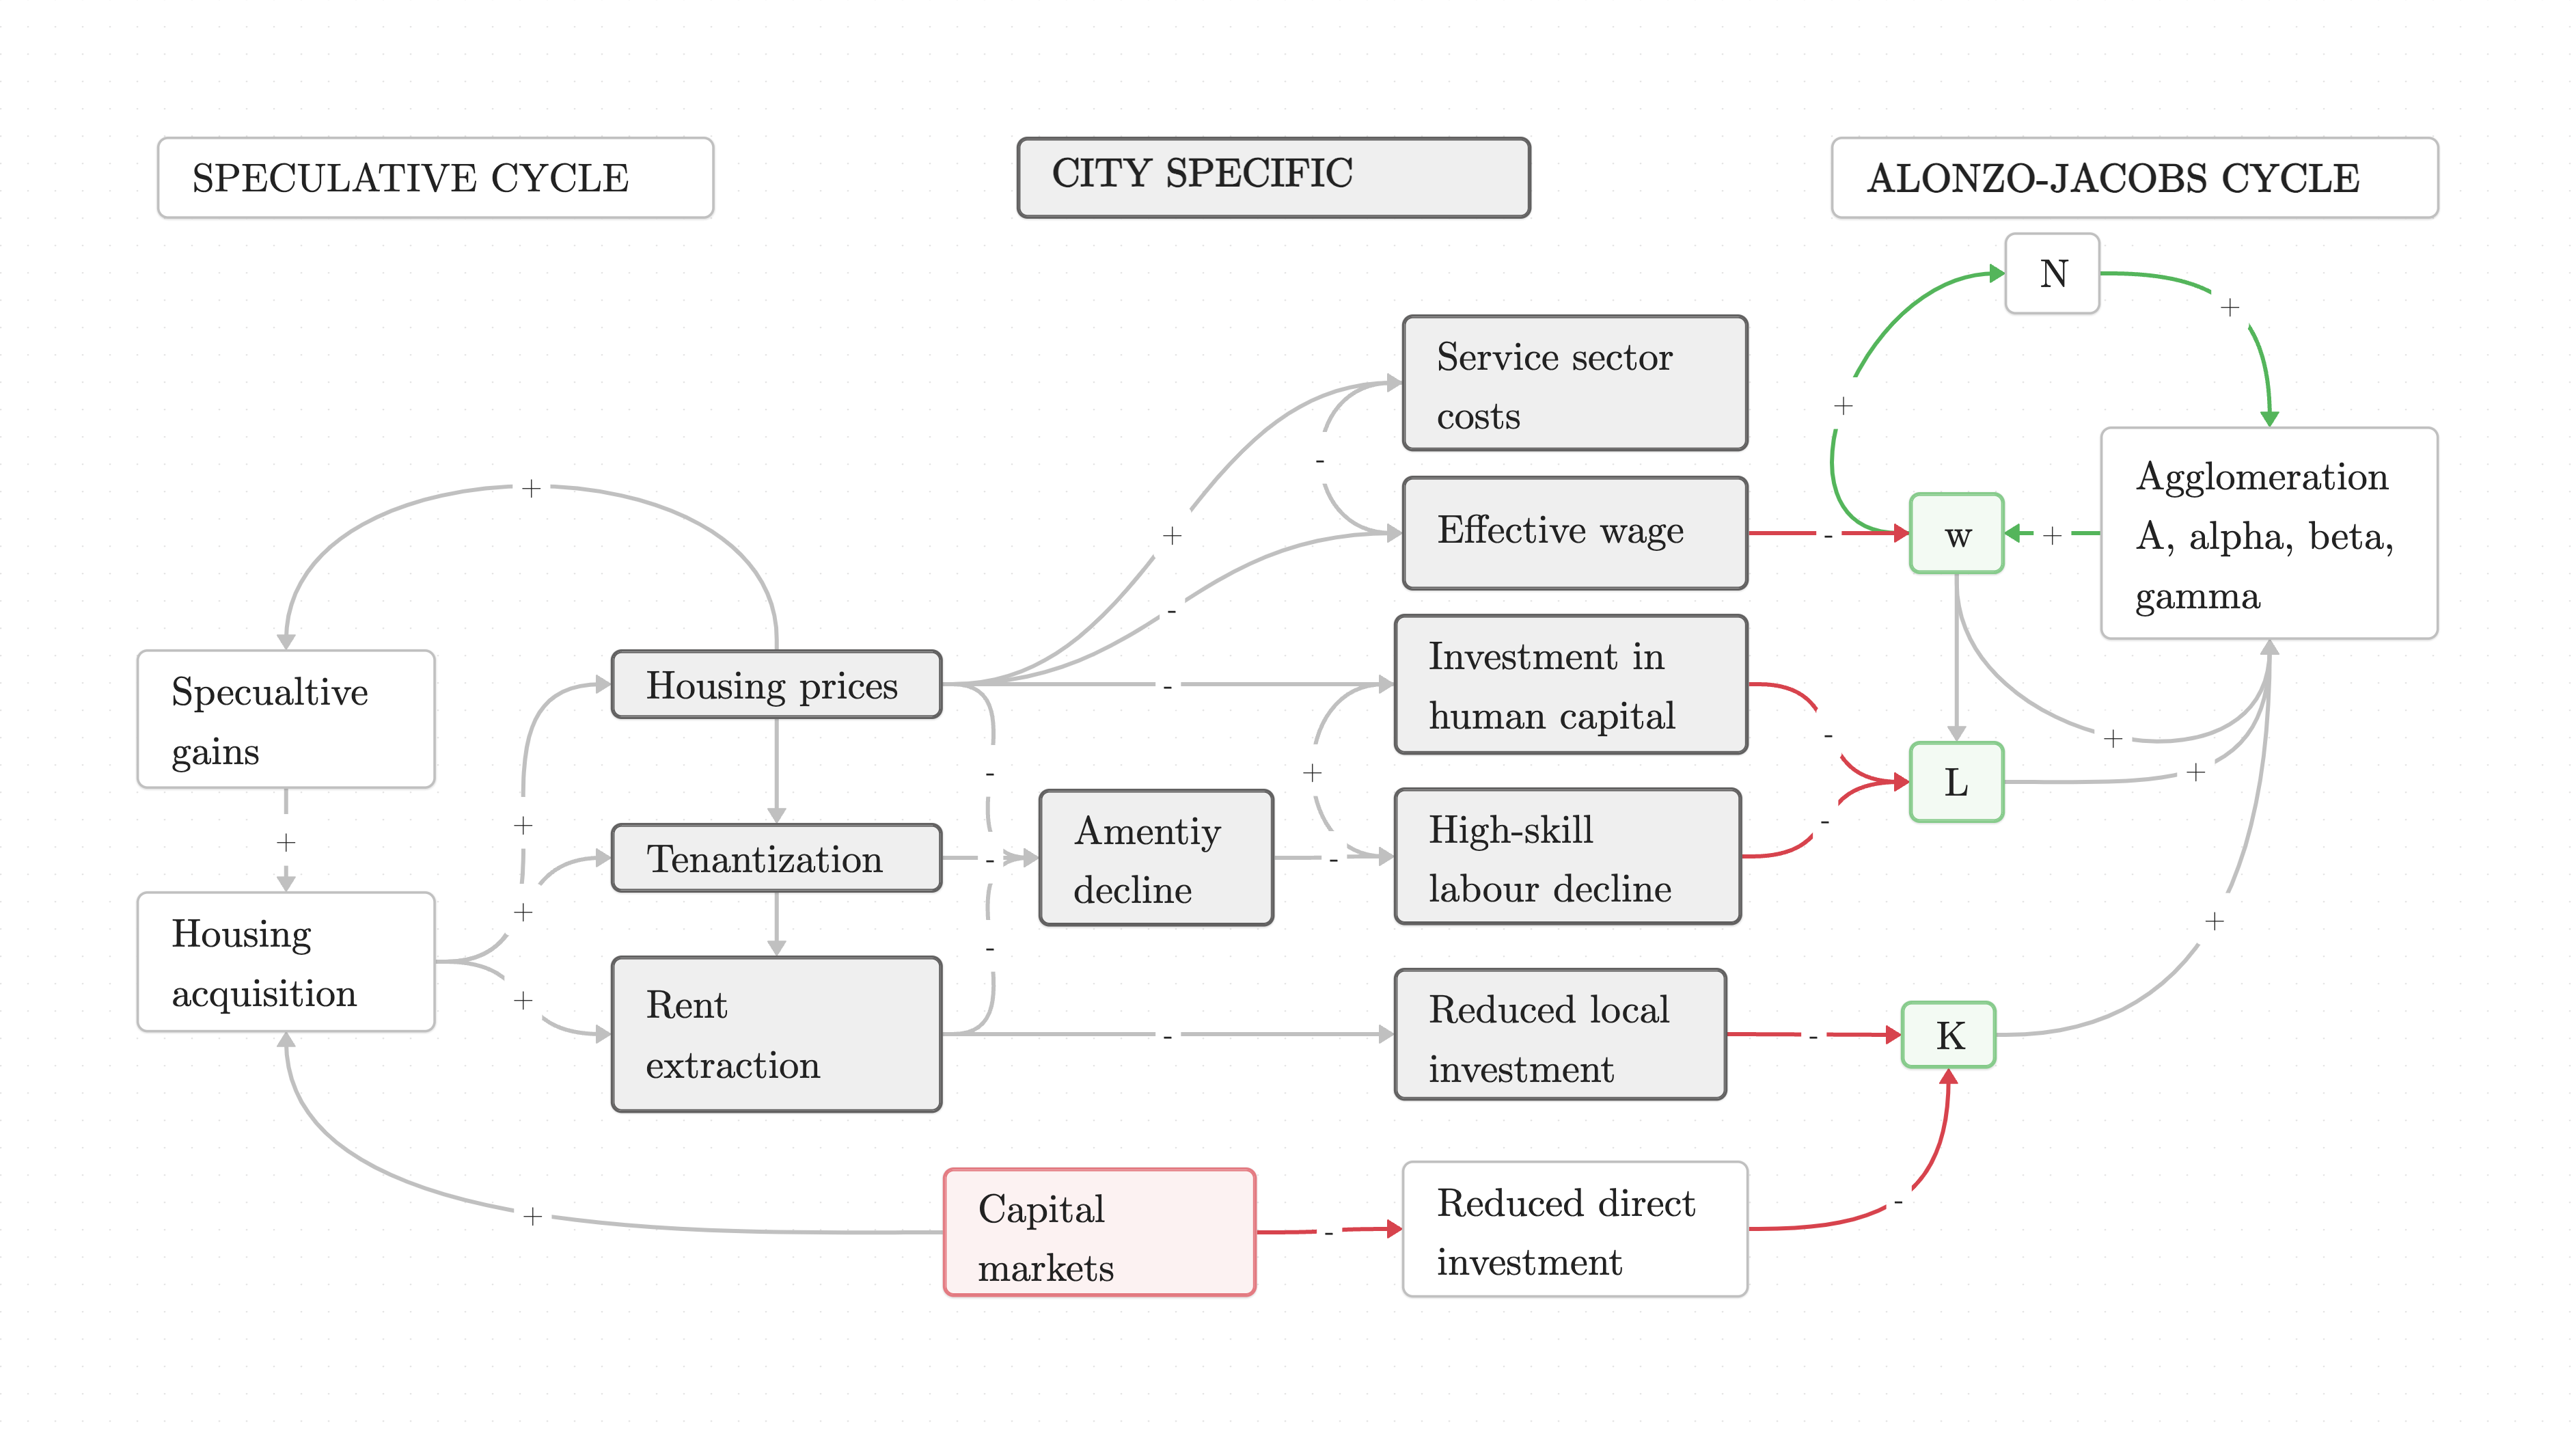
\includegraphics[scale=.15 ]{fig/impact-channels.png}%angle=90
\end{adjustwidth}
\caption{Impact channels relating financialization and urban productivity.}
\end{figure}
%}

This experiment indicates that policy parameters are likely to affect the ownership trajectory in different ways when there is a link between financialization and urban productivity and when there is no link.